\documentclass[8pt]{beamer}
\usetheme{Montpellier}
\usecolortheme{beaver}
%\usetheme{Antibes}
%\usecolortheme{dolphin}

\usepackage[utf8]{inputenc}
\usepackage[T1]{fontenc}
\usepackage[french]{babel}
\usepackage{lmodern}
\usepackage{amsmath}
\usepackage{amssymb}
\usepackage{mathrsfs}
\usepackage{bm}
\usepackage[load-configurations = abbreviations]{siunitx}
\usepackage{graphicx}
\usepackage{epstopdf}
\usepackage[]{animate}
\usepackage[lofdepth,lotdepth]{subfig}
\usepackage[justification=centering]{caption}
\usepackage{wrapfig}
\usepackage{multirow}
\usepackage{eurosym}
\usepackage{enumitem}
\usepackage{url}
\usepackage{multimedia}
\usepackage[normalem]{ulem}
\usepackage{tikz}
\usepackage{tikz-3dplot}
\usetikzlibrary{shapes}

\setbeamertemplate{navigation symbols}{}
\addtobeamertemplate{navigation symbols}{}{%
	\usebeamerfont{footline}%
	\usebeamercolor[fg]{footline}%
	\hspace{1em}%
	\hfill\insertframenumber%/\inserttotalframenumber
}
\setbeamertemplate{itemize item}[ball]

\graphicspath{{./images/}}

% spécifie le domaine d'un plot tikz avec {_}{_} plutôt que _:_
\tikzset{domaine/.style 2 args={domaine=#1:#2}}
% anime des dessins tikz
\tikzset{invisible/.style={opacity=0},
		 visible on/.style={alt={#1{}{invisible}}},
		 alt/.code args={<#1>#2#3}{\alt<#1>{\pgfkeysalso{#2}}{\pgfkeysalso{#3}}}}

\def\doubleunderline#1{\underline{\underline{#1}}}

\newcommand{\dd}[2]{\cfrac{\mathrm{d} #1}{\mathrm{d} #2}}
\newcommand{\ddt}[1]{\dd{#1}{t}}
\newcommand{\ddelta}[2]{\cfrac{\partial #1}{\partial #2}}

\newcommand{\makecube}[1]{
	\coordinate (A#1) at (.5,-.5,-.5) ; \coordinate (B#1) at (.5,.5,-.5) ;
	\coordinate (C#1) at (-.5,.5,-.5) ; \coordinate (D#1) at (-.5,-.5,-.5) ;
	\coordinate (Ab#1) at (.5,-.5,.5) ; \coordinate (Bb#1) at (.5,.5,.5) ;
	\coordinate (Cb#1) at (-.5,.5,.5) ; \coordinate (Db#1) at (-.5,-.5,.5) ;
	\draw (Ab#1) -- (A#1) -- (B#1) -- (C#1) -- (Cb#1) -- (Db#1) -- (Ab#1) -- (Bb#1) -- (Cb#1) ;
	\draw (Bb#1) -- (B#1) ;
}

\newcommand{\makecubedashed}[1]{
	\coordinate (A#1) at (.5,-.5,-.5) ; \coordinate (B#1) at (.5,.5,-.5) ;
	\coordinate (C#1) at (-.5,.5,-.5) ; \coordinate (D#1) at (-.5,-.5,-.5) ;
	\coordinate (Ab#1) at (.5,-.5,.5) ; \coordinate (Bb#1) at (.5,.5,.5) ;
	\coordinate (Cb#1) at (-.5,.5,.5) ; \coordinate (Db#1) at (-.5,-.5,.5) ;
	\draw (Ab#1) -- (A#1) -- (B#1) -- (C#1) -- (Cb#1) -- (Db#1) -- (Ab#1) -- (Bb#1) -- (Cb#1) ;
	\draw (Bb#1) -- (B#1) ;
	\draw[densely dashed] (A#1) -- (D#1) -- (C#1) ; \draw[densely dashed] (D#1) -- (Db#1);
}

\title{Imagerie 3D et simulation numérique pour l'étude multi-échelles de la compression d'une poudre constituée de grains déformables}
\subtitle{Soutenance de thèse}
\author{Maxime \textsc{Teil}}
\date{09 décembre 2019}

\begin{document}

{\setbeamertemplate{navigation symbols}{}
\begin{frame}[plain]
	\begin{center}
		{\small Soutenance de thèse de Maxime \textsc{Teil}}\vspace{.01\textwidth}\\
		{\footnotesize Contrat doctoral de l'école doctorale IMEP2 - Université Grenoble Alpes}\vspace{.03\textwidth}\\
		{\color[rgb]{0.,0,0.5}{\LARGE Imagerie 3D et simulation numérique pour l'étude multi-échelles de la compression d'une poudre constituée de grains déformables}}\vspace{.05\textwidth}\\
		{\small Le 09 décembre 2019}\vspace{.03\textwidth}\\
		{\small En présence de :}\vspace{.04\textwidth}\\
		\begin{minipage}[c]{0.32\textwidth}\centering
			{\small Saïd \textsc{El Youssoufi}}\\
			{\small Jean-Philippe \textsc{Ponthot}}\\
			(Rapporteurs)
		\end{minipage}
		\begin{minipage}[c]{0.32\textwidth}\centering
			{\small Anne-Sophie \textsc{Caro-Bretelle}}
			{\small Pascal \textsc{Villard}}\\
			(Examinateurs)
		\end{minipage}
		\begin{minipage}[c]{0.32\textwidth}\centering
			{\small Barthélémy \textsc{Harthong}}\\
			{\small Didier \textsc{Imbault}}\\
			{\small Robert \textsc{Peyroux}}\\
			(Encadrants)
		\end{minipage}
		\vspace{.05\textwidth}
	\end{center}
	\begin{tikzpicture}[remember picture, overlay]
		\pgfmathsetmacro{\figsize}{.12}
		\pgfmathsetmacro{\figspace}{.03}
		\node[above right=2mm] (labo) at (current page.south west) {
			\includegraphics[height=\figsize\textwidth]{logos/3sr.eps}\hspace{\figspace\textwidth}
			\includegraphics[height=\figsize\textwidth]{logos/uga.eps}\hspace{\figspace\textwidth}
			\includegraphics[height=\figsize\textwidth]{logos/GrenobleINP.eps}\hspace{\figspace\textwidth}
			\includegraphics[height=\figsize\textwidth]{logos/cnrs.png}};
	\end{tikzpicture}
\end{frame}
\addtocounter{framenumber}{-1}
}

\begin{frame}
	\frametitle{Plan de la soutenance}
	\tableofcontents
\end{frame}

\section[Projet de thèse]{Présentation du projet de thèse}
\begin{frame}
	\frametitle{Plan de la soutenance}
	\tableofcontents[currentsection]
\end{frame}

\subsection{Travaux antérieurs}
\begin{frame}
	\frametitle{Projet scientifique}
	\vfill
	\begin{block}{Projet COMPACT - Institut Carnot PolyNat - 2014/2015}
		\'Etude de la mise en forme d'un matériau biosourcé à partir de grains natifs d'amidon.
	\end{block}\vfill
	\begin{center}
	\begin{tikzpicture}[scale=1.]
		\node[] (amidon) at (-3,0) {\includegraphics[height=2.5cm]{projet/amidon.png}};
		\node[] (sample) at (3,0) {\includegraphics[width=3.5cm]{projet/sample_thermo.png}};
		\draw[->, thick] (amidon) -- (sample) node [midway, above] {Thermo-compression\footnotemark[1]};
	\end{tikzpicture}\\\vfill
	\begin{minipage}[c]{.6\textwidth}
		\begin{block}{Deux phases dans le même temps :}
			\begin{itemize}[label=$\rightarrow$]
				\item La compression de la poudre dans une matrice ;
				\item Le soudage des grains par transfert de chaleur.
			\end{itemize}
		\end{block}
	\end{minipage}
	\begin{minipage}[c]{.39\textwidth}\centering
		\begin{tikzpicture}[scale=.4]
			% dessine les plateaux chauffants
			\draw[] (-4.5,-2) rectangle (4.5,-3);
			\draw[] (-4.5,2) rectangle (4.5,3);
			\path (0,-2.5) node {Plateau chauffant};
			\path (0,2.5) node {Plateau chauffant};
			% dessine le moule inférieur
			\filldraw[fill=gray!70] (-4.2,-0.5) rectangle (4.2, -2);
			% dessine le moule supérieur
			\filldraw[fill=gray!70] (-4.2,2) -- (4.2, 2) -- ++(0,-1.4) -- ++(-1.2,0) -- ++(0,-1) -- ++(-6,0) -- ++(0,1) -- ++(-1.2,0) -- cycle;
			\path (0,1) node {Moule};
			% dessine les grains
			\filldraw[dashed, white, fill=white!90!blue] (-3,-0.7) rectangle (3,-1.5);
			\path (0,-1.05) node {Grains};
			% Compression
			\foreach \t in {-4,-3,...,4} {
				\draw[-stealth, blue, ultra thick] (\t,3.8) -- ++(0,-.8);
				\draw[-stealth, blue, ultra thick] (\t,-3.8) -- ++(0,.8);
			}
			% Chauffage
			\fill[red!80!gray, opacity=.7] (-4.5,-2) rectangle (4.5,-3);
			\fill[red!80!gray, opacity=.7] (-4.5,2) rectangle (4.5,3);
			\fill[fill=red!80!gray, opacity=.2] (-4.2,-0.5) rectangle (4.2, -2);
			\fill[fill=red!80!gray, opacity=.2] (-4.2,2) -- (4.2, 2) -- ++(0,-1.4) -- ++(-1.2,0) -- ++(0,-1) -- ++(-6,0) -- ++(0,1) -- ++(-1.2,0) -- cycle;
		\end{tikzpicture}
	\end{minipage}
	\vfill
	\end{center}\vfill
	\footnotetext[1]{A. Regazzi \textit{et al.}, Composites Science and Technology, 2019}
\end{frame}
\begin{frame}
	\frametitle{Travaux réalisés avant la thèse - Problématique}
	\vfill
	\begin{minipage}[c]{.29\textwidth}\centering
		\includegraphics[width=.9\textwidth]{projet/fissure.png}
	\end{minipage}
	\begin{minipage}[c]{.7\textwidth}
	\begin{block}{Analyse des pièces fracturées :}
		\begin{itemize}[label=$\rightarrow$]
			\item Propriétés mécaniques dépendantes de l'état de densité ;
			\item Changement de phase observé dans certaines régions ;
			\item Hétérogénéité des morphologies selon l'épaisseur.
		\end{itemize}
	\end{block}
	\end{minipage}\\\vfill
	\begin{block}{Problématique}
		Il est nécessaire de comprendre le comportement thermique et mécanique en compression d'un ensemble de grains déformables dont les géométries sont complexes et variées.
	\end{block}\vfill
	\begin{block}{Stratégie}
		\begin{itemize}[label=$\rightarrow$]
			\item \alt<2>{\textbf{Développer un outil qui permet d'étudier la compression des grains en tenant compte de l'hétérogénéité de la microstructure et de son évolution ;}}{Développer un outil qui permet d'étudier la compression des grains en tenant compte de l'hétérogénéité de la microstructure et de son évolution ;}
			\item \alt<2>{{\color{gray}Intégration du couplage thermo-mécanique.}}{Intégration du couplage thermo-mécanique.}
		\end{itemize}
	\end{block}\vfill
\end{frame}

\subsection{Objectif des travaux de thèse}
\begin{frame}
	\frametitle{\'Etude de la phase de compression d'une poudre polymère}
	\vfill
	\begin{block}{Objectifs}
		Utiliser une méthode numérique pour simuler la densification du milieu granulaire en considérant :
		\begin{itemize}[label=$\rightarrow$]
			\item le caractère déformable des grains constituant le milieu ;
			\item la géométrie réelle des grains ;
			\item l'évolution réelle de la microstructure.
		\end{itemize}
	\end{block}\vfill\centering
	\textbf{\`A partir du comportement mécanique individuel des grains, connaître le comportement mécanique à l'échelle d'un VER.}\\\vfill
	\textbf{Développer un algorithme optimisé permettant l'automatisation et l'utilisation de la méthode qui est validée par l'expérience.}\\
	\vfill
\end{frame}

\subsection{Méthodes}
\begin{frame}
	\frametitle{Méthode expérimentale et numérique}
	\begin{minipage}[c]{.35\textwidth}
		\begin{itemize}[label=$\rightarrow$]
			\item<1-> Création d'un échantillon numérique ;
			\\
			\item<2-> Enregistrement de la microstructure ;
			\\
			\item<3-> Utilisation de l'expérience pour créer la simulation ;
			\\
			\item<3-> Simulation sur un sous-volume : comportement mécanique mésoscopique.
		\end{itemize}
	\end{minipage}
	\begin{minipage}[c]{.64\textwidth}\centering
	\begin{tikzpicture}[scale=1.]
		\tdplotsetmaincoords{75}{125}
		\uncover<2->{
			\node (tomo) at (1.5,3) {\includegraphics[width=3cm]{3D_samples/1MPa/3D_0.jpg}};
			\path (tomo.north) ++(0,-0.15) node [above] {Tomographie};
			\begin{scope}[shift={(1.6,3)}, scale=.2, tdplot_main_coords]
			\makecube{A}
			\end{scope}
			\draw[dashed] (AA) -- (-0.3,0); \draw[dashed] (BA) -- (1.4,-0.7);
			\draw (AbA) -- (-0.25,1.65); \draw (BbA) -- (1.65,1.3);}
		\node (grain) at (3.1,-1) {\includegraphics[width=2.5cm]{grain.png}};
		\node (set) at (0,0) {\includegraphics[width=3.5cm]{set.png}};
		\draw (grain) circle (1.4); \draw (set) ++(0.4,-0.25) circle (0.5);
		\uncover<3->{
			\node (dvc) at (4,2) {\includegraphics[width=2cm]{3D_dispZ_2MPa/3D_Uz_10.jpg}};
			\path (dvc.north) ++(0,-0.15) node [above] {Corrélation 3D};}
	\end{tikzpicture}
	\end{minipage}
\end{frame}
\begin{frame}
	\frametitle{Matériau granulaire étudié}
	\begin{block}{Le polystyrène comme matériau modèle}
		Compte tenu des capacités du tomographe du laboratoire, une poudre de polystyrène a été choisie comme matériau modèle :
		\begin{itemize}[label=$\rightarrow$]
			\item taille de grains de l'ordre de \SI{150}{\micro\meter} (\SI{20}{\micro\meter} pour l'amidon);
			\item géométrie des grains très complexe ;
			\item composition polymérique ;
			\item propriétés mécaniques similaires à celles de grains d'amidon.
		\end{itemize}
		Fournisseur : Goodfellow (UK) -
		Référence : ST316051/4
	\end{block}
	\centering
	\includegraphics[width=0.35\textwidth]{projet/PS_300x300.jpg}
\end{frame}
\begin{frame}
	\frametitle{Imagerie 3D - Tomographie à rayons X}
	\begin{minipage}[c]{0.7\textwidth}
		\begin{animateinline}[autoplay, loop, palindrome]{2}
			\multiframe{18}{iangle=0+10}{
				\tdplotsetmaincoords{70}{110}
				\begin{tikzpicture}[scale=1.]
					% Source RX
					\fill[gray!70] (-5,0.5) rectangle (-3,-0.5);
					\fill[gray!70] (-3,0.2) rectangle (-2.8,-0.2);
					\draw[] (-5,0.5) rectangle (-3,-0.5) ; \draw[] (-3,0.2) rectangle (-2.8,-0.2);
					\path (-7.8/2,-0.8) node [] {Source rayons X};
					% Echantillon
					\begin{scope}[xshift=-0.2cm, tdplot_main_coords]
						\path[tdplot_screen_coords] (0,-1.5) node []{\'Echantillon};
						\coordinate (orig) at (0,0,-1);
						\draw[] (0,0,1) circle (0.5);
						\tdplotdrawarc[, dashed]{(0,0,-1)}{0.5}{110}{290}{}{}
						\tdplotdrawarc[]{(0,0,-1)}{0.5}{290}{470}{}{}
						\tdplotsetrotatedcoordsorigin{(orig)}
						\tdplotsetthetaplanecoords{110}
						\draw[tdplot_rotated_coords] (0,0.5,0) -- (2,0.5,0);
						\tdplotsetthetaplanecoords{290}
						\draw[tdplot_rotated_coords] (0,0.5,0) -- (2,0.5,0);
						\tdplotsetrotatedcoords{\iangle}{0}{0}
						\draw[tdplot_rotated_coords, ->, red] (orig) -- (1,0,0);
						\draw[tdplot_rotated_coords, ->, green] (orig) -- (0,1,0);
						\draw[tdplot_rotated_coords, ->, blue] (orig) -- (0,0,2.5);
						\draw[opacity=0.] (-1,-1,-1) -- (1,1,1.5);
					\end{scope}
					% Detecteur
					\draw[ultra thick] (1.5,2) -- (1.5,-2);
					\path (1.5,-2.3) node {Détecteur};
					% rayons X
					\fill[opacity=.3, green!70!orange] (-2.8,0) -- (1.5,2) -- (1.5,-2) -- cycle;
					% echantillon 3D
					\node (3d_sample) at (-3.5,-3.5) {\includegraphics[width=2.5cm]{3D_0_00.png}};
					% projection 3d
					\begin{scope}[shift={(4,-4)}, scale=0.7, tdplot_main_coords]
						\draw[opacity=0.] (-2,-2,-2) -- (2,2,2);
						\tdplotsetthetaplanecoords{\iangle}
						\draw[tdplot_rotated_coords, thick, fill=gray!50] (-2,-1.2,0) -- ++(4,0,0) -- ++(0,2.4,0) -- ++(-4,0,0) -- cycle;
						\foreach \t in {0,10,...,170} {
							\tdplotsetthetaplanecoords{\t}
							\draw[tdplot_rotated_coords, color=gray] (-2,-1.2,0) -- ++(4,0,0) -- ++(0,2.4,0) -- ++(-4,0,0) -- cycle;
						}
					\end{scope}
					% projections vers 3d
					\draw[->, thick] (3,-4) -- (-2,-4) node[midway, above] {Assemblage et reconstruction} ;
				\end{tikzpicture}
			}
		\end{animateinline}
	\end{minipage}
	\begin{minipage}[t]{.29\textwidth}\centering
		\animategraphics[width=\textwidth, autoplay, loop, palindrome]{2}{biblio/proj/proj_}{00}{17}\\
		\vspace{.02\textwidth}
		Projections
	\end{minipage}
\end{frame}
\begin{frame}
	\frametitle{Corrélation de volumes - Calcul de la cinématique}
	Utilisation du code TomoWarp2\footnotemark[1] permettant la corrélation d'images 3D par une méthode de recherche d'imagettes 3D.\vspace{.03\textwidth}\\
	\centering
	\begin{tikzpicture}[scale=1.]
		\path (0,0) node {\includegraphics[width=3cm, height=3cm]{biblio/PS_2D.jpg}};
		\draw[red, thick] (-1.5,-1.5) grid [step=.5cm] (1.5,1.5);
		\uncover<2-3>{
		\fill[red, opacity=.5] (-1.5,-1.5) rectangle ++(.5,.5);
		}
		\begin{scope}[shift={(6,0)}, scale=1.]
			\pgfmathsetmacro{\xshift}{0.6}
			\pgfmathsetmacro{\yshift}{0.9}
			\path (\xshift,\yshift) node {\includegraphics[width=3cm, height=3cm]{biblio/PS_2D.jpg}};
			\draw[red, thick] (-1.5,-1.5) grid [step=.5cm] (1.5,1.5);
			\uncover<2>{
				\fill[orange, opacity=.5] (-1.5-1,-1.5-1) rectangle ++(2.5,2.5);
				\fill[red, opacity=.5] (-1.5,-1.5) rectangle ++(.5,.5);
			}
			\uncover<3>{
				\draw[orange] (-1.5-1,-1.5-1) rectangle ++(2.5,2.5);
				\fill[red, opacity=.5] (-1.5,-1.5) rectangle ++(.5,.5);
				\filldraw[green, fill opacity=.5, shift={(\xshift,\yshift)}] (-1.5,-1.5) rectangle ++(.5,.5);
			}
			\uncover<4>{
				\draw[green, thick, shift={(\xshift,\yshift)}] (-1.5,-1.5) grid [step=.5cm] (1.5,1.5);
				\draw[very thick, -latex] (1.5,-1.5) -- ++(\xshift,0) node [midway, below] {$u$};
				\draw[very thick, -latex] (1.5+\xshift,-1.5) -- ++(0,\yshift) node [midway, right] {$v$};
			}
		\end{scope}
		\draw [->, thick] (1.8,0.5) -- (4.2,0.5) node [midway, above] {Mouvement};
	\end{tikzpicture}\\
	Illustration en 2D d'un mouvement de corps rigide
	\footnotetext[1]{E. Tudisco \textit{et al.}, SoftwareX, 2017}
\end{frame}

\begin{frame}
	\frametitle{Méthodes numériques - Simulation des milieux granulaires}
	\vfill
	\begin{block}{Méthode des éléments discrets (DEM)}
		Inconvénient : difficulté à traduire la déformation des éléments.	
	\end{block}\vfill
	\begin{block}{Méthode des éléments finis (FEM)}
		Inconvénient : adaptée aux milieux continus.
	\end{block}\vfill
	\begin{block}{Méthode des éléments finis multi-particules (MP-FEM)}
	\begin{minipage}[c]{.49\textwidth}
	Adaptée à l'étude des milieux continus constituant les particules d'un milieu granulaire et leur déformation.\\
	\null\\
	Gestion des interactions de surface dans les zones de contact.\\
	\end{minipage}
	\begin{minipage}[c]{.49\textwidth}\centering
		%\animategraphics[autoplay, loop, width=.95\textwidth]{4}{illustration_nouha/simu_}{00}{25}
		\animategraphics[autoplay, loop, timeline=timelineMPFEM.tln, width=.95\textwidth]{4}{illustration_nouha/simu_}{00}{25}
	\end{minipage}
	\end{block}
	\vfill
\end{frame}

\section[Travaux expérimentaux]{Travaux expérimentaux}
\begin{frame}
	\frametitle{Plan de la soutenance}
	\tableofcontents[currentsection]
\end{frame}
\subsection{Compression triaxiale}
\begin{frame}
	\frametitle{Essai de compression triaxiale de révolution}
	\begin{block}{Cellule de chargement triaxial}
	\centering
	\vfill
	\begin{minipage}[c]{.69\textwidth}\centering
		\includegraphics[width=.99\textwidth]{triax/triax_bis.eps}
	\end{minipage}
	\begin{minipage}[c]{0.29\textwidth}\centering
		\includegraphics[width=\textwidth]{triax/photo_dispo.jpg}
	\end{minipage}
	\vfill
	\end{block}
	\begin{tikzpicture}[remember picture, overlay]
		\path (current page.center) ++(-4.2,1.2) coordinate (A);
		\node [draw, text width=3.2cm] (pilotage) at (A) {\textbf{Pilotage :}\\Pression de confinement\\Déplacement axial};
	\end{tikzpicture}
\end{frame}
\begin{frame}
	\frametitle{Protocole expérimental}
	\vfill
	\begin{block}{Mise en place de l'essai}
		\centering
		\begin{tikzpicture}[scale=1.]
			\node (A) at (0,0) {\includegraphics[height=3cm]{triax/proc00.jpg}};
			\node (B) at (2.55,0) {\includegraphics[height=3cm]{triax/proc01.jpg}};
			\node (C) at (5.28,0) {\includegraphics[height=3cm]{triax/proc02.jpg}};
			\node (D) at (7.34,0) {\includegraphics[height=3cm]{triax/proc03.jpg}};
			\node (E) at (9.23,0) {\includegraphics[height=3cm]{triax/proc04.jpg}};
			\node[draw, fill=white, below right=.15cm] (a) at (A.north west) {a};
			\node[draw, fill=white, below right=.15cm] (b) at (B.north west) {b};
			\node[draw, fill=white, below right=.15cm] (c) at (C.north west) {c};
			\node[draw, fill=white, below right=.15cm] (d) at (D.north west) {d};
			\node[draw, fill=white, below right=.15cm] (e) at (E.north west) {e};
		\end{tikzpicture}\\
		\hfill
		\begin{minipage}[t]{.45\textwidth}
			a) Mise en place de la membrane\\
			b) Introduction dans le moule\\
			c) Remplissage dans la membrane
		\end{minipage}
		\hfill
		\begin{minipage}[t]{.45\textwidth}
			d) Retrait du moule\\
			e) Insertion dans la cellule
		\end{minipage}\hfill
	\end{block}\vfill
	\begin{minipage}[c]{0.69\textwidth}
		\vfill
		\begin{block}{\'Echantillon}
			\begin{minipage}[c]{.49\textwidth}\centering
				Hauteur : $\approx \SI{22}{\milli\meter}$
			\end{minipage}
			\begin{minipage}[c]{.49\textwidth}\centering
				Diamètre : \SI{10}{\milli\meter}
			\end{minipage}
		\end{block}\vfill
		\begin{block}{Déroulement de l'essai}
			\begin{itemize}[label=$\rightarrow$]
				\item Vitesse de chargement axial : \SI[per-mode=symbol]{2}{\micro\meter\per\second}
				\item Déformation logarithmique axiale finale : $\approx$ \num{.25}
			\end{itemize}
		\end{block}\vfill
	\end{minipage}
	\begin{minipage}[c]{.29\textwidth}\centering
		\begin{tikzpicture}
			\path (0,0) node[below] {\includegraphics[width=1cm]{triax/membrane_0.png}};
			\path (1.2,0) node[below] {\includegraphics[width=1cm]{triax/membrane_1.png}};
			\path (2.4,0) node[below] {\includegraphics[width=1cm]{triax/membrane_2.png}};
		\end{tikzpicture}
	\end{minipage}\\\vfill
\end{frame}
\begin{frame}
	\frametitle{Campagne d'essais}
	\vfill
	\begin{block}{Plusieurs pressions de confinement}
		Trois essais ont été menés à trois pressions de confinement différentes :
		\begin{center}
		\begin{itemize}[label=$\rightarrow$]
			\item $P_C = \SI{1}{\mega\pascal}$
			\item $P_C = \SI{2}{\mega\pascal}$
			\item $P_C = \SI{7}{\mega\pascal}$
		\end{itemize}
		\end{center}
	\end{block}\vfill
	\begin{minipage}[c]{.65\textwidth}\centering
		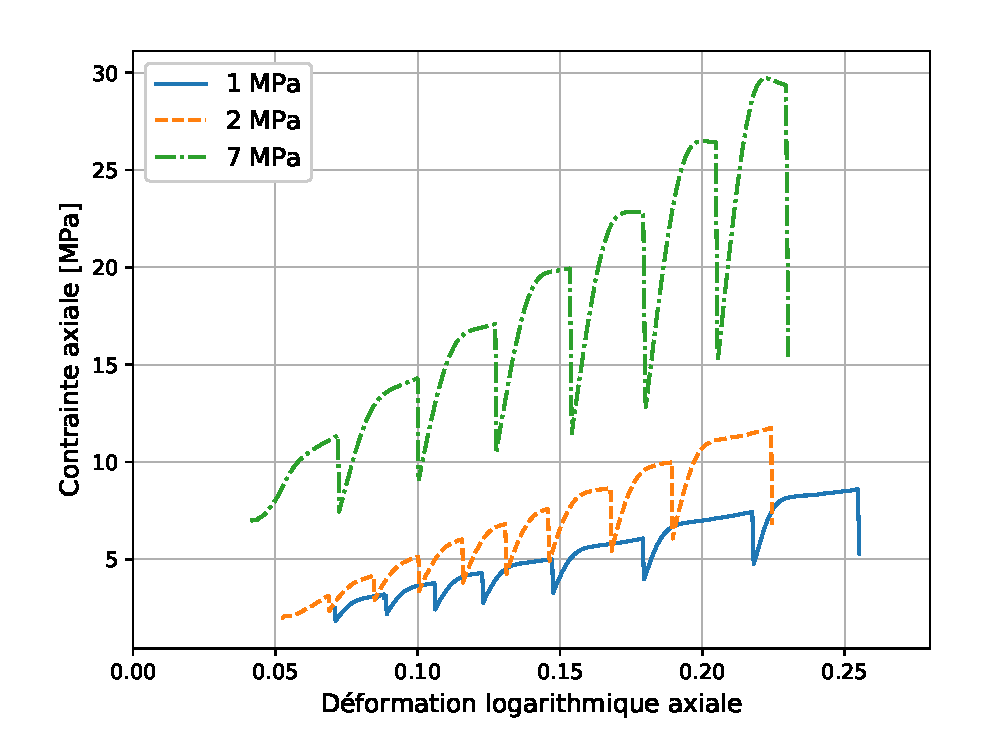
\includegraphics[width=\textwidth]{triax/stress_strain.eps}
	\end{minipage}
	\begin{minipage}[c]{.34\textwidth}
		\begin{block}{\'Etats successifs de compression}
			Caractérisation par tomographie à chaque relaxation.\\
			\null\\
			\'Etats successifs suffisamment proches afin de permettre la corrélation d'images 3D.
		\end{block}
	\end{minipage}\\
	\vfill
	\begin{tikzpicture}[remember picture, overlay, scale=1.]
		\coordinate (O) at (current page.center);
		\path (O) ++ (-4.55,-4.22) node {{\tiny $\bigstar$}};
		% tomo 1MPa
		\path (O) ++ (-3.05,-4) node [blue] {{\tiny $\bigstar$}};
		\path (O) ++ (-2.7,-3.95) node [blue] {{\tiny $\bigstar$}};
		\path (O) ++ (-2.35,-3.9) node [blue] {{\tiny $\bigstar$}};
		\path (O) ++ (-2,-3.85) node [blue] {{\tiny $\bigstar$}};
		\path (O) ++ (-1.45,-3.8) node [blue] {{\tiny $\bigstar$}};
		\path (O) ++ (-.8,-3.75) node [blue] {{\tiny $\bigstar$}};
		\path (O) ++ (0,-3.6) node [blue] {{\tiny $\bigstar$}};
		\path (O) ++ (0.75,-3.5) node [blue] {{\tiny $\bigstar$}};
		% tomo 2MPa
		\path (O) ++ (-3.5,-4) node [orange] {{\tiny $\bigstar$}};
		\path (O) ++ (-3.1,-3.95) node [orange] {{\tiny $\bigstar$}};
		\path (O) ++ (-2.8,-3.88) node [orange] {{\tiny $\bigstar$}};
		\path (O) ++ (-2.45,-3.8) node [orange] {{\tiny $\bigstar$}};
		\path (O) ++ (-2.15,-3.75) node [orange] {{\tiny $\bigstar$}};
		\path (O) ++ (-1.8,-3.65) node [orange] {{\tiny $\bigstar$}};
		\path (O) ++ (-1.5,-3.55) node [orange] {{\tiny $\bigstar$}};
		\path (O) ++ (-1.05,-3.47) node [orange] {{\tiny $\bigstar$}};
		\path (O) ++ (-0.6,-3.37) node [orange] {{\tiny $\bigstar$}};
		\path (O) ++ (0.15,-3.27) node [orange] {{\tiny $\bigstar$}};
%		% tomo 7MPa
		\path (O) ++ (-3.7,-3.28) node [green] {{\tiny $\bigstar$}};
		\path (O) ++ (-3.05,-3.15) node [green] {{\tiny $\bigstar$}};
		\path (O) ++ (-2.45,-2.93) node [green] {{\tiny $\bigstar$}};
		\path (O) ++ (-1.90,-2.73) node [green] {{\tiny $\bigstar$}};
		\path (O) ++ (-1.35,-2.58) node [green] {{\tiny $\bigstar$}};
		\path (O) ++ (-.8,-2.38) node [green] {{\tiny $\bigstar$}};
		\path (O) ++ (-.28,-2.08) node [green] {{\tiny $\bigstar$}};
		\path (O) ++ (.25,-1.95) node [green] {{\tiny $\bigstar$}};
		% Legende
		\path (O) ++ (1.5,1) node {$\bigstar$ : Scan de tomographie};
	\end{tikzpicture}
\end{frame}

\subsection{Tomographie}
\begin{frame}
	\frametitle{Compression triaxiale in-situ}
	\centering\vfill
	\includegraphics[width=\textwidth]{tomo/in_situ.pdf}
	\vfill
	Résolution maximale permettant une taille de voxel de \SI{9}{\micro\meter}.
	\vfill
\end{frame}

\subsection{Corrélation d'images 3D}
\begin{frame}
	\frametitle{Corrélation de volumes - Utilisation de TomoWarp2}
	\vfill
	\centering
	Le code TomoWarp2\footnotemark[1], a été utilisé pour les calculs de corrélation d'images volumiques entre chaque état de compression successif.
	\vfill{\centering
	\begin{tikzpicture}[scale=1.]
		\path (-3,0) node {\includegraphics[width=4cm]{DVC/deplacement.png}};
		\path (3,0) node {\includegraphics[width=4cm]{DVC/deformation.png}};
		\draw [-stealth] (-1,0) -- (1,0) node[midway, above] {Green-Lagrange};
		\path (-3,2.5) node {Champs de déplacement};
		\path (3,2.5) node {Champs de déformation};
	\end{tikzpicture}}
	\vfill
	\footnotetext[1]{E. Tudisco \textit{et al.}, SoftwareX, 2017}
\end{frame}
\begin{frame}
	\frametitle{Déplacement dans l'échantillon}
	\centering
	\begin{tikzpicture}[scale=1.]
		\pgfmathsetmacro{\xshift}{2.5}
		\pgfmathsetmacro{\yshift}{-2.5}
		\node (a) at (0,0) {\includegraphics[width=2cm]{DVC/suivi/0.jpg}};
		\node (b) at (\xshift,0) {\includegraphics[width=2cm]{DVC/suivi/1.jpg}};
		\node (c) at (2*\xshift,0) {\includegraphics[width=2cm]{DVC/suivi/2.jpg}};
		\node (d) at (3*\xshift,0) {\includegraphics[width=2cm]{DVC/suivi/3.jpg}};
		\node (e) at (3*\xshift,\yshift) {\includegraphics[width=2cm]{DVC/suivi/5.jpg}};
		\node (f) at (2*\xshift,\yshift) {\includegraphics[width=2cm]{DVC/suivi/7.jpg}};
		\node (g) at (\xshift,\yshift) {\includegraphics[width=2cm]{DVC/suivi/9.jpg}};
		\node (h) at (0,\yshift) {\includegraphics[width=2cm]{DVC/suivi/10.jpg}};
		\draw[->, thick] (a) -- (b) ; \draw[->, thick] (b) -- (c) ; \draw[->, thick] (c) -- (d) ;
		\draw[->, thick] (d) -- (e) ; \draw[->, thick] (e) -- (f) ; \draw[->, thick] (f) -- (g) ;
		\draw[->, thick] (g) -- (h) ;
		\node[draw, fill=white, below right=.1cm] (A) at (a.north west) {Initial};
		\node[draw, fill=white, below right=.1cm] (B) at (b.north west) {Confinement};
		\node[draw, fill=white, below right=.1cm] (C) at (c.north west) {1er arrêt};
		\node[draw, fill=white, below right=.1cm] (D) at (d.north west) {2ème arrêt};
		\node[draw, fill=white, below right=.1cm] (E) at (e.north west) {4ème arrêt};
		\node[draw, fill=white, below right=.1cm] (F) at (f.north west) {6ème arrêt};
		\node[draw, fill=white, below right=.1cm] (G) at (g.north west) {7ème arrêt};
		\node[draw, fill=white, below right=.1cm] (H) at (h.north west) {Fin};
		\node[text width=2.3cm, minimum height=2cm, text centered] (leg) at (0,2*\yshift) {$P_C=\SI{1}{\mega\pascal}$ Pris au milieu de l'échantillon};
		\coordinate (Im1) at (1.7*\xshift,2*\yshift);
		\path (Im1) ++(1.3,0) coordinate (Im2);
		\node[left] (im) at (Im1) {\includegraphics[height=2.5cm]{3D_samples/1MPa/3D_0.jpg}};
		\node[right] (im2) at (Im2) {\includegraphics[height=2.5cm]{3D_samples/1MPa/3D_9.jpg}};
		\draw [->, thick] (Im1) -- ++(1.3,0);
		\begin{scope}[shift={(1.18*\xshift,2*\yshift+0.2)}, scale=.15, red]
			\makecube{A}
		\end{scope}
		\begin{scope}[shift={(2.78*\xshift,2*\yshift-0.3)}, scale=.15, yscale=0.8, red]
			\makecube{B}
		\end{scope}
	\end{tikzpicture}
\end{frame}

\section[Traitement numérique]{Traitement numérique de l'imagerie 3D}
\begin{frame}
	\frametitle{Plan de la soutenance}
	\tableofcontents[currentsection]
\end{frame}
\subsection{Retouche des images 3D}
\begin{frame}
	\frametitle{Amélioration des images issues de tomographie}
	\vfill
	\begin{block}{Image d'origine}
		De manière générale, l'image issue directement de la reconstruction de tomographie présente :
		\begin{itemize}[label=$\rightarrow$]
			\item un signal bruité (détecteur, expérience, méthode d'acquisition, ...)
			\item des artefacts liés à la reconstruction ("ring")
		\end{itemize}
	\end{block}\vfill
	\begin{minipage}[c]{.39\textwidth}\centering
		\includegraphics[width=\textwidth]{ameliorations_images/00-orig_0142.jpg}
	\end{minipage}
	\begin{minipage}[c]{.59\textwidth}\centering
		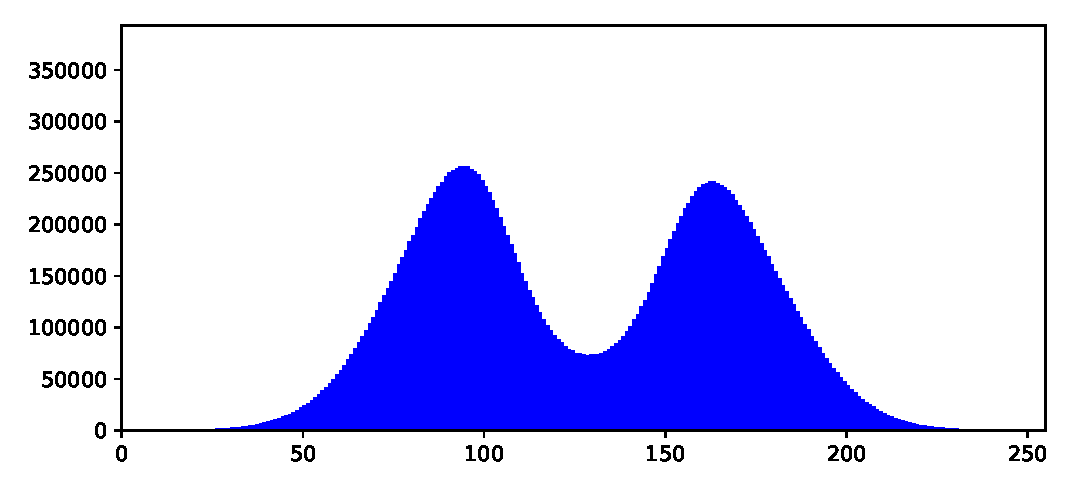
\includegraphics[width=\textwidth]{ameliorations_images/00-orig_hist.eps}
	\end{minipage}\\\vfill
	\begin{tikzpicture}[remember picture, overlay]
		\coordinate (O) at (current page.center);
		\draw [->, thick] (O) ++ (-0.5,-3.6) -- ++(5.65,0) node [midway, below] {{\small Niveaux de gris}};
		\draw [->, thick] (O) ++ (5.15,-3.22) -- ++(0,2.48) node [above, text width=1cm] {{\small Nombre de voxel}};
		\path (O) ++(-0.4,-1.) node[draw, right] {{\small Histogramme}};
	\end{tikzpicture}
\end{frame}
\begin{frame}
	\frametitle{Amélioration des images issues de tomographie}
	\vfill
	\begin{block}{Image d'origine}
		\begin{minipage}[c]{.29\textwidth}\centering
			\includegraphics[width=\textwidth]{ameliorations_images/00-orig_0142.jpg}
		\end{minipage}
		\begin{minipage}[c]{.69\textwidth}\centering
			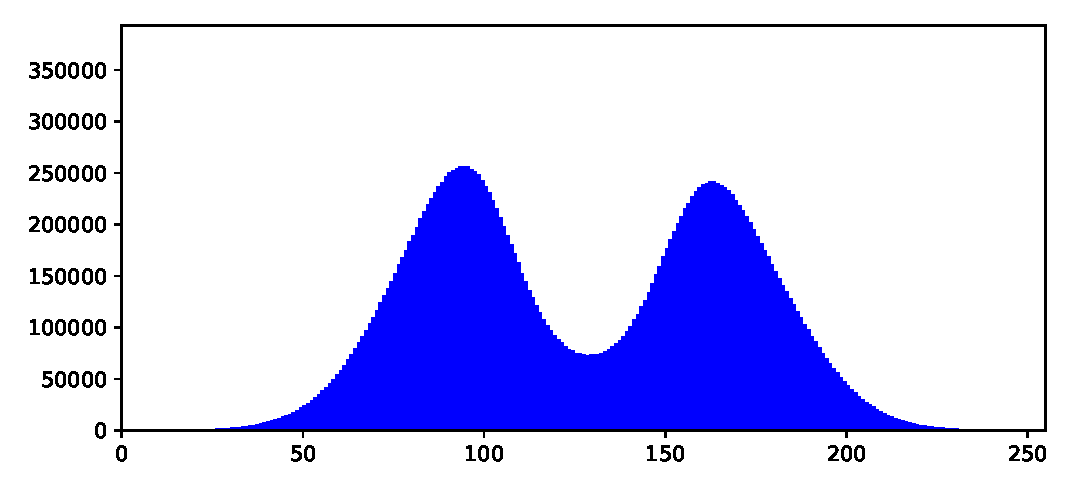
\includegraphics[width=\textwidth]{ameliorations_images/00-orig_hist.eps}
		\end{minipage}
	\end{block}
	\vfill
	\begin{block}{Réajustement du contraste + Atténuation (bilatéral + Variation totale)}
		\begin{minipage}[c]{.29\textwidth}\centering
			\includegraphics[width=\textwidth]{ameliorations_images/03-bilatTV_0142.jpg}
		\end{minipage}
		\begin{minipage}[c]{.69\textwidth}\centering
			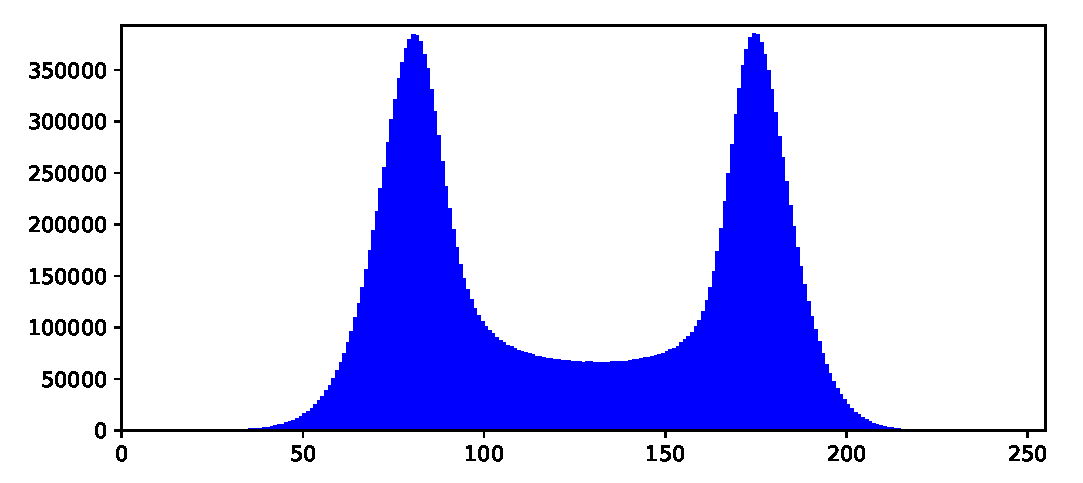
\includegraphics[width=\textwidth]{ameliorations_images/03-bilatTV_hist.eps}
		\end{minipage}
	\end{block}\vfill
\end{frame}

\subsection{Processus de segmentation}
\begin{frame}
	\frametitle{Seuillage automatique - Segmentation biphasique}
	\begin{block}{Seuillage automatique}
		Le seuillage automatique permet d'identifier différentes phases dans une image à partir des intensités de voxels en niveaux de gris et du type de signal (histogramme).\\
		Dans le cas d'une image représentant deux phases, deux méthodes sont réputées :
		\begin{itemize}[label=$\rightarrow$]
			\item La méthode d'Otsu\footnotemark[1] donne une valeur de seuillage $S_O$
			\item La méthode de Kittler\footnotemark[2] donne une valeur de seuillage $S_K$
		\end{itemize}
		\vspace{.02\textwidth}
		Les deux méthodes fonctionnent correctement mais ne s'accordent pas sur la valeur du seuillage ($S_O \neq S_K$).\vspace{.02\textwidth}\\
		Une moyenne pondérée entre les deux méthodes est réalisée :
		$$
		S = \alpha\times S_O + (1-\alpha)\times S_K
		$$
	\end{block}
	\footnotetext[1]{N. Otsu, \textit{IEEE Transactions on Systems, Man, and Cybernetics}, 9, 1979}
	\footnotetext[2]{J. Kittler et J. Illingworth, \textit{Pattern Recognition}, 19, 1986}
\end{frame}
\begin{frame}
	\frametitle{Seuillage automatique - Segmentation biphasique}
	\centering
	$ S = \alpha\times S_O + (1-\alpha)\times S_K $\vspace{.02\textwidth}\\
	\begin{minipage}[c]{.32\textwidth}\centering
		$\alpha = 1.0$ [Otsu]\\
		\includegraphics[width=.85\textwidth]{threshold/contour_120_0142.png}
	\end{minipage}
	\begin{minipage}[c]{.32\textwidth}\centering
		${\color{red}\boxed{\alpha = 0.4}}$\\
		\includegraphics[width=.85\textwidth]{threshold/contour_126_0142.png}
	\end{minipage}
	\begin{minipage}[c]{.32\textwidth}\centering
		$ \alpha = 0.0$ [Kittler]\\
		\includegraphics[width=.85\textwidth]{threshold/contour_130_0142.png}
	\end{minipage}\vspace{.01\textwidth}\\
	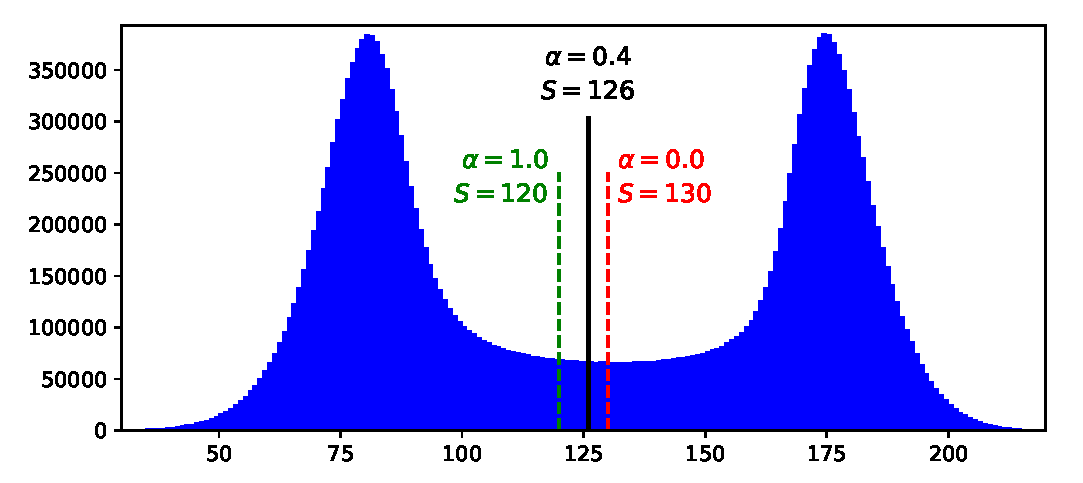
\includegraphics[width=.75\textwidth]{threshold/histogram.eps}
	\begin{tikzpicture}[remember picture, overlay]
		\coordinate (O) at (current page.center);
		\path (O) ++(4,2.7) node[draw, fill=white] {Appréciation visuelle};
	\end{tikzpicture}
\end{frame}
\begin{frame}
	\frametitle{Segmentation - Objectif}
	\vfill
	\begin{block}{C'est quoi ?}
		La séparation et l'identification des particules.
	\end{block}\vfill
	\begin{block}{Comment ?}
		En attribuant à chaque voxel un label qui dépend de la particule considérée.
	\end{block}\vfill
	\begin{block}{Pourquoi ?}
		Sélectionner des particules et les analyser et/ou les extraire.
	\end{block}\vfill
	\begin{block}{Quelques difficultés}
		\begin{minipage}[t]{.29\textwidth}
			\begin{itemize}[label=$\rightarrow$]
				\item Contacts
				\item Faible résolution
				\item Diffusion
				\item[] ...
			\end{itemize}
		\end{minipage}
		\begin{minipage}[t]{.70\textwidth}
			\begin{itemize}[label=$\rightarrow$]
				\item Les grains n'ont pas une forme régulière et convexe
				\item Les grains peuvent avoir des porosités internes
				\item Le milieu peut être très polydisperse
			\end{itemize}
		\end{minipage}
	\end{block}
	\vfill
	\begin{tikzpicture}[remember picture, overlay]
		\coordinate (O) at (current page.center);
		\path (O) ++(1.7,2) node {\includegraphics[width=2cm]{segm/grid/grid_orig.png}};
		\path (O) ++(4.8,2) node {\includegraphics[width=2cm]{segm/grid/grid_label.png}};
		\draw[->, very thick] (O) ++(2.8,2) -- ++(.9,0);
		\path (O) ++(4,-1) node {\includegraphics[width=2cm]{segm/grid/grid_postlabel.png}};
		\path (O) ++(4.2,-1.1) node [draw, fill=white] {{\small $A=4\text{vx}$}};
	\end{tikzpicture}
\end{frame}
\begin{frame}
	\frametitle{Segmentation - Watershed}
	\begin{block}{Propagation des marqueurs - Watershed}
		Image $\Leftrightarrow$ Carte topographique\\
		Propagation des marqueurs $\Leftrightarrow$ \'Elévation des eaux
		\begin{itemize}[label=$\rightarrow$]
			\item<2-> Un marqueur $=$ un nombre $=$ un minimum $=$ un lac
			\item<3-> Propagation des marqueurs qui dépend du voisinage $=$ crue qui dépend de l'altitude
			\item<4-> Quand deux marqueurs se rencontrent, il y a toujours deux marqueurs $=$ création de digues artificielles
			\item<5-> Les marqueurs se propageant ne peuvent pas atteindre une valeur seuil $=$ haut plateau
		\end{itemize}
	\end{block}
	\centering
	\begin{tikzpicture}[scale=1.]
		\node (img) at (0,0) {\includegraphics[width=3cm]{segm/bilattv_0045.jpg}};
		\coordinate (A) at (-0.41,0.85); \coordinate(B) at (-0.27,0.28);
		\coordinate (C) at (-0.15,-0.2); \coordinate (D) at (0.05,-1.);
		\draw [red, very thick, dashed, ->] (-0.6,1.6) -- (0.2,-1.6);
		\uncover<2>{
			\draw [orange, line width=0.1cm] (A) -- ++(104:0.15); \draw [orange, line width=0.1cm] (A) -- ++(180+104:0.15);
			\draw [blue, line width=0.1cm] (B) -- ++(104:0.05); \draw [blue, line width=0.1cm] (B) -- ++(180+104:0.05);
			\draw [green, line width=0.1cm] (C) -- ++(104:0.02); \draw [green, line width=0.1cm] (C) -- ++(180+104:0.02);
			\draw [purple, line width=0.1cm] (D) -- ++(104:0.25); \draw [purple, line width=0.1cm] (D) -- ++(180+104:0.25);}
		\uncover<3>{
			\draw [orange, line width=0.1cm] (A) -- ++(104:0.25); \draw [orange, line width=0.1cm] (A) -- ++(180+104:0.28);
			\draw [blue, line width=0.1cm] (B) -- ++(104:0.15); \draw [blue, line width=0.1cm] (B) -- ++(180+104:0.08);
			\draw [green, line width=0.1cm] (C) -- ++(104:0.05); \draw [green, line width=0.1cm] (C) -- ++(180+104:0.05);
			\draw [purple, line width=0.1cm] (D) -- ++(104:0.40); \draw [purple, line width=0.1cm] (D) -- ++(180+104:0.28);}
		\uncover<4>{
			\draw [orange, line width=0.1cm] (A) -- ++(104:0.28); \draw [orange, line width=0.1cm] (A) -- ++(180+104:0.35);
			\draw [blue, line width=0.1cm] (B) -- ++(104:0.25); \draw [blue, line width=0.1cm] (B) -- ++(180+104:0.09);
			\draw [green, line width=0.1cm] (C) -- ++(104:0.08); \draw [green, line width=0.1cm] (C) -- ++(180+104:0.06);
			\draw [purple, line width=0.1cm] (D) -- ++(104:0.50); \draw [purple, line width=0.1cm] (D) -- ++(180+104:0.30);}
		\uncover<5>{
			\draw [orange, line width=0.1cm] (A) -- ++(104:0.35); \draw [orange, line width=0.1cm] (A) -- ++(180+104:0.35);
			\draw [blue, line width=0.1cm] (B) -- ++(104:0.25); \draw [blue, line width=0.1cm] (B) -- ++(180+104:0.15);
			\draw [green, line width=0.1cm] (C) -- ++(104:0.12); \draw [green, line width=0.1cm] (C) -- ++(180+104:0.10);
			\draw [purple, line width=0.1cm] (D) -- ++(104:0.55); \draw [purple, line width=0.1cm] (D) -- ++(180+104:0.38);}
		\begin{scope}[shift={(3,-1.3)}, scale=1.]
			\uncover<2>{
				\fill [orange] (0.4,0.1) rectangle (1.56,.9);
				\fill [blue] (1.56,0.1) rectangle (2.28,.9);
				\fill [green] (2.3,0.1) rectangle (2.9,.9);
				\fill [purple] (2.9,0.1) rectangle (4.5,.9);}
			\uncover<3>{
				\fill [orange] (0.4,0.1) rectangle (1.56,1.2);
				\fill [blue] (1.56,0.1) rectangle (2.28,1.2);
				\fill [green] (2.3,0.1) rectangle (2.9,1.2);
				\fill [purple] (2.9,0.1) rectangle (4.5,1.2);}
			\uncover<4>{
				\fill [orange] (0.4,0.1) rectangle (1.56,1.5);
				\fill [blue] (1.56,0.1) rectangle (2.28,1.5);
				\fill [green] (2.3,0.1) rectangle (2.9,1.5);
				\fill [purple] (2.9,0.1) rectangle (4.5,1.5);
				\draw[thick] (1.56,0.1) -- (1.56,1.5);}
			\uncover<5>{
				\fill [orange] (0.4,0.1) rectangle (1.56,1.7);
				\fill [blue] (1.56,0.1) rectangle (2.28,1.7);
				\fill [green] (2.3,0.1) rectangle (2.9,1.7);
				\fill [purple] (2.9,0.1) rectangle (4.5,1.7);
				\draw[thick] (1.56,0.1) -- (1.56,1.7);}
			\fill[gray] plot[xscale=.05, yscale=.01] file {plotProfileFill.txt};
			\draw plot[xscale=.05, yscale=.01] file {plotProfile.txt};
			\draw [red, very thick, dashed, ->] (-0.05,0) -- ++(4.75,0) node[midway, below] {Direction de la coupe};
			\draw [->, thick] (0,0) -- ++(0,2.5) node[above] {Niveaux de gris};
			\uncover<5>{\draw[very thick, densely dotted] (-0.1,1.7) -- (4.7,1.7);}
		\end{scope}
	\end{tikzpicture}
	%\includegraphics[width=.5\textwidth]{segm/explain/watershed.png}
\end{frame}
\begin{frame}
	\frametitle{Segmentation - Maxima locaux et Watershed}
	\vfill
	\begin{tikzpicture}[scale=1.]\centering
		\path (0,0) node {\includegraphics[width=4cm]{segm/explain/not_easy/new_seeds_illustration.jpg}};
		\uncover<1>{
			\node [draw, below] (explain) at (5.5,2) {Recherche des maxima locaux};
			\path (5.5,0.8) node [text width=6.5cm, text centered] {
					Application d'un filtre maximum\\(dilatation sur l'image en niveaux de gris);};
			\path (5.5,-0.2) node [text width=6.5cm, text centered] {
					Différence entre l'image d'origine et l'image dilatée;};
			\path (5.5,-1.2) node [text width=6.5cm, text centered] {
					Maxima locaux $=$ différence nulle.};}
		\uncover<2>{
			\path (7,0) node {\includegraphics[width=4cm]{segm/explain/not_easy/ws.jpg}};
			\draw [->, thick] (2.25,0) -- (4.75,0) node [midway, above] {Watershed};}
	\end{tikzpicture}
	\vfill\centering
	\only<1>{
		\vfill\centering
		\begin{tikzpicture}[scale=1.]
			\node (gray) at (0,0) {\includegraphics[width=3cm]{segm/explain/maxima_locaux/gray_flou.png}};
			\node (maximum) at (3.5,0) {\includegraphics[width=3cm]{segm/explain/maxima_locaux/maximum_50.png}};
			\node (superpose) at (7,0) {\includegraphics[width=3cm]{segm/explain/maxima_locaux/gray_flou.png}};
			\path (superpose) node {\includegraphics[width=3cm]{segm/explain/maxima_locaux/maxima_alpha.png}};
		\end{tikzpicture}
	}
	\uncover<2>{
	\begin{minipage}[t]{.45\textwidth}
		\begin{block}{Avantages}
			\begin{itemize}[label=$\rightarrow$]
				\item Les plus petites particules ne sont pas oubliées ;
				\item Capacité de trouver des particules avec de grandes zones de contact.
			\end{itemize}
		\end{block}
	\end{minipage}
	\begin{minipage}{.08\textwidth}
		~
	\end{minipage}
	\begin{minipage}[t]{.45\textwidth}
		\begin{block}{Inconvénient}
			\begin{itemize}[label=$\rightarrow$]
				\item Nombre de particules surestimé.
			\end{itemize}
		\end{block}
	\end{minipage}
	}
	\vfill
\end{frame}
\begin{frame}
	\frametitle{Segmentation - Correction des contacts}
	\vfill
	\begin{block}{Détection et analyse de chaque paire de contact}
		Pour une paire de contact entre les labels $A$ et $B$, on définit :
		\begin{itemize}[label=$\rightarrow$]
			\item $N_A$ (resp. $N_B$) le nombre de voxels caractérisant la surface du grain $A$ (resp. B) ;
			\item $N_C(A,B)$ le nombre de voxels caractérisant la surface de contact entre les deux particules.
		\end{itemize}
		Une condition est utilisée pour déterminer la nature du contact et corriger la segmentation :
		$$\boxed{
		\text{Si}\quad
		\cfrac{N_C(A,B)}{\min(N_A, N_B)} > S_C
		\quad\text{alors}\quad
		A = B
		}$$
	\end{block}\vfill
	\centering
	\begin{tikzpicture}[scale=1.]
		\path (0,0) node {\includegraphics[width=3cm]{segm/explain/not_easy/ws.jpg}};
		\path (7,0) node {\includegraphics[width=3cm]{segm/explain/not_easy/ws_correct.jpg}};
		\draw [->, thick] (1.75,0) -- (5.25,0) node [midway, above] {Correction} node [midway, below] {des contacts};
	\end{tikzpicture}
	\vfill
\end{frame}
\begin{frame}
	\frametitle{Segmentation - Résultats sur les images de tomographie}
		\vfill
		\begin{center}
		Le choix des paramètres de segmentation est qualitatif et se base sur la comparaison visuelle de l'image segmentée avec celle issue de la tomographie.\\\vfill
		\begin{tikzpicture}[scale=1.]
			\node (orig) at (0,-2) {\includegraphics[width=3cm]{segm/200_orig.jpg}};
			\node (segm) at (8,-2) {\includegraphics[width=3cm]{segm/200_label.jpg}};
			\node (superpose) at (4,0) {\includegraphics[width=3cm]{segm/200_superpose.jpg}};
			\node [draw, ellipse, blue] (choix) at (4,-2) {$S_C = 0.15$};
			\node [text width=3.5cm, text centered] (choix bis) at (4,-3) {Les surfaces de contact ne sont pas plus grandes que \SI{15}{\percent} de la surface totale du plus petit grain.};
			\draw [->, thick] (orig) -- (superpose);
			\draw [->, thick] (segm) -- (superpose);
		\end{tikzpicture}
		\end{center}
		\vfill
\end{frame}
\begin{frame}
	\frametitle{Segmentation - Résultats sur les images de tomographie}
	\centering
	\begin{minipage}[c]{.34\textwidth}\centering
		\textbf{Volume représenté :}\\
		829 grains\\
		$140 \times 140 \times 140$ [$\text{vx}^3$]\\
		15 Mo\\
		~\\
		\textbf{Temps pour le traitement :}\\
		\SI{3.5}{\second}\\
		~\\
		\textbf{Temps pour la segmentation :}\\
		\SI{3}{\minute} et \SI{45}{\second}\\
		~\\
		\uncover<2>{{\color{blue}
		\textbf{Temps pour la génération du maillage:}\\
		\SI{36}{\minute}\\
		~\\
		\textbf{Simulation :}\\
		4 jours et \SI{3}{\hour}\\
		26 Go}}\\
	\end{minipage}
	\begin{minipage}[c]{.64\textwidth}\centering
		\includegraphics[width=\textwidth]{segm/segmentation_3D.png}
	\end{minipage}\\
\end{frame}

\subsection{Génération d'un maillage}
\begin{frame}
	\frametitle{Utilisation du mailleur iso2mesh (Matlab/Octave)}
	\hfill
	Le mailleur \emph{iso2mesh}\footnotemark[1] basé sur un langage de programmation Matlab/Octave permet de générer des maillages surfaciques ou volumiques à partir d'images 3D.\\\vfill
	\begin{minipage}[t]{.45\textwidth}\centering
		\begin{block}{\centering Entrée}\centering
			Image 3D améliorée\\
			en niveaux de gris\\
			\includegraphics[width=.6\textwidth]{mesh/label16_resized.png}
		\end{block}
	\end{minipage}
	\begin{minipage}{.08\textwidth}
		\null
	\end{minipage}
	\begin{minipage}[t]{.45\textwidth}\centering
		\begin{block}{\centering Sortie}\centering
			Maillage volumique\\
			constitué de tétraèdres\\
			\includegraphics[width=.7\textwidth]{mesh/03_s2m_resized.png}
		\end{block}
	\end{minipage}\\\vfill
	\begin{tikzpicture}[remember picture, overlay]
		\coordinate (O) at (current page.center);
		\path (O) ++(-5,-2) node [draw] {\num{4300} voxels};
		\path (O) ++(+4.8,-1.7) node [draw] {\num{2384} éléments};
		\path (O) ++(+4.8,-2.3) node [draw] {\num{528} n\oe{}uds};
	\end{tikzpicture}
	\footnotetext[1]{Fang et Boas, \textit{2009 IEEE International Symposium on Biomedical Imaging: From Nano to Macro}, 2009.}
\end{frame}
\begin{frame}
	\frametitle{Processus de maillage}
	\vfill
	\begin{block}{Génération du maillage dans \emph{iso2mesh} :}
		\begin{itemize}[label=$\rightarrow$]
			\item Création, réparation, nettoyage et simplification d'un maillage surfacique ;
			\item Génération d'un maillage volumique à partir du maillage surfacique ;
			\item Enregistrement de la liste des n\oe{}uds et table de connectivité.
		\end{itemize}
	\end{block}\vfill
	\begin{block}{Création d'éléments quadratiques}\centering
		\begin{minipage}[t]{.49\textwidth}\centering
		\begin{tikzpicture}[scale=.5]
			\coordinate (A) at (0,0,0);
			\coordinate (B) at (9,1,6);
			\coordinate (C) at (8,0,0);
			\coordinate (D) at (6,4,2);
			\draw[<-, >=stealth, dashed] (14/3,4/3,2/3) to[bend right=25] ++(-1,1.5,0) node[above left]{Face 4};
			\draw[dashed] (A) node[left]{1} node{$\bullet$} -- (C) node[right]{3} node{$\bullet$};
			\draw[<-, >=stealth, dashed] (17/3,1/3,2) to[bend left=50] ++(-1,-1,0) node[left]{Face 1};
			\draw (A) -- (B) node[below]{2} node{$\bullet$};
			\draw (A) -- (D) node[above]{4} node{$\bullet$};
			\draw (B) -- (C);
			\draw (B) -- (D);
			\draw (C) -- (D);
			\draw[<-, >=stealth] (5,5/3,8/3) to[bend right=15] ++(-2,1,0) node[left]{Face 2};
			\draw[<-, >=stealth] (23/3,5/3,8/3) to[bend right=30] ++(1.2,1.2,0) node[above]{Face 3};
		\end{tikzpicture}
	\end{minipage}
	\begin{minipage}[t]{.49\textwidth}\centering
		\begin{tikzpicture}[scale=.5]
			\coordinate (A) at (0,0,0);
			\coordinate (B) at (9,1,6);
			\coordinate (C) at (8,0,0);
			\coordinate (D) at (6,4,2);
			\draw[dashed] (A) node[left]{1} node{$\bullet$} to[bend left=10] node[color=blue,pos=0.5]{$\bullet$} node[color=blue,pos=0.5,above]{7} (C) node{$\bullet$} node[right]{3};
			\draw (A) to[bend left=8] node[color=blue,pos=0.5]{$\bullet$} node[color=blue,pos=0.5,below]{5} (B) node[below]{2} node{$\bullet$};
			\draw (A) to[bend right=10] node[color=blue,pos=0.5]{$\bullet$} node[color=blue,pos=0.5,above left]{8} (D) node[above]{4} node{$\bullet$};
			\draw (B) to[bend right=30] node[color=blue,pos=0.5]{$\bullet$} node[color=blue,pos=0.5,below right]{6} (C);
			\draw (B) to[bend right=5] node[color=blue,pos=0.5]{$\bullet$} node[color=blue,pos=0.5,right]{9} (D);
			\draw (C) to[bend right=15] node[color=blue,pos=0.5]{$\bullet$} node[color=blue,pos=0.5,above right]{10} (D);
		\end{tikzpicture}
	\end{minipage}
	\end{block}\vfill
\end{frame}
\begin{frame}
	\frametitle{Modification du volume des grains maillés}
	\vfill
	\begin{block}{Objectifs :}
		\begin{itemize}[label=$\rightarrow$]
			\item \'Eviter les changements de volume liés aux phases de segmentation et de maillage ;
			\item Lorsque les grains sont introduits dans une simulation, permettre une densité apparente initiale du milieu la plus proche possible de celle mesurée dans l'échantillon réel.
		\end{itemize}
		\begin{center}
			\textbf{$\Rightarrow$ Générer des contacts initiaux pour la simulation.}
		\end{center}
	\end{block}\vfill
	\begin{block}{Effet de la génération du maillage - \'Echelle du grain}
		$$
		\forall \text{grain},\qquad
		\cfrac{\left|V_\text{segmenté}^\text{grain}-V_\text{maillé}^\text{grain}\right|}{V_\text{segmenté}^\text{grain}} > \SI{0.1}{\percent}
		\quad\Rightarrow\quad\text{homothétie}
		$$
	\end{block}\vfill
	\begin{block}{Effet de la segmentation - \'Echelle de l'ensemble de grains}
		$$
		\cfrac{\left|V_\text{seuillé}^\text{ensemble}-V_\text{maillé}^\text{ensemble}\right|}{V_\text{seuillé}^\text{ensemble}} > \SI{0.1}{\percent}
		\quad\Rightarrow\quad\text{homothétie}
		$$
	\end{block}\vfill
\end{frame}

\section[Simulations numériques]{Simulations numériques}
\begin{frame}
	\frametitle{Plan de la soutenance}
	\tableofcontents[currentsection]
\end{frame}

\subsection{Conditions initiales}
\begin{frame}
	\frametitle{Mise en place de l'échantillon numérique}
	\vfill
	\begin{block}{Lors de la segmentation}
		\begin{itemize}[label=$\rightarrow$]
			\item Enregistrement des positions des boîtes qui englobent chaque grain segmenté.
		\end{itemize}
	\end{block}\vfill
	\begin{block}{Dans Abaqus}
		\begin{itemize}[label=$\rightarrow$]
			\item Insertion des grains maillés aux positions enregistrées lors de la phase de segmentation.
		\end{itemize}
	\end{block}
	\vfill
	\centering
	\begin{tikzpicture}[scale=1.]
		\draw[opacity=0.] (-7.5,-2.6) rectangle (2.25,2.3);
		\path (0,0) node {\includegraphics[width=4.5cm]{3D_samples/1MPa/3D_0.jpg}};
		\tdplotsetmaincoords{70}{110}
		\begin{scope}[scale=.5, tdplot_main_coords, color=red]
			\makecube{A}
		\end{scope}
		\path (-5,0.05) node {\includegraphics[width=.45\textwidth]{3D_local_abaqus.png}};
		\fill[red, opacity=.3] (AbA) -- (-2.5,2.3) -- (-2.5,-2.2) -- (AA);
		\draw[red, thick] (AbA) -- (-2.5,2.3);
		\draw[red, thick] (AA) -- (-2.5,-2.2);
		\draw[red, thick] (-2.5,2.3) rectangle (-7.5,-2.2);
		\node[draw, color=red, fill=white] (Vmeso) at (-5,-2.05) {Volume mésoscopique};
	\end{tikzpicture}
	\vfill
\end{frame}
\begin{frame}
	\frametitle{Définition du matériau et contacts}
	\vfill
	\begin{block}{Loi de comportement élastoplastique avec écrouissage isotrope}
		Caractéristiques moyennes issues des éléments de la littérature\footnotemark[1].
	\end{block}\vfill
	\begin{block}{Gestion des contacts inter-granulaires}
		\begin{itemize}[label=$\rightarrow$]
			\item Coefficient de friction PS-PS$^{1,}$\footnotemark[2] : \num{.5}
			\item Pas de cohésion des contacts
		\end{itemize}
	\end{block}\vfill
	\begin{block}{Gestion des contacts initiaux}
		\centering
		~\\
		\begin{tikzpicture}[scale=1.]
			\begin{scope}[scale=.7]
				\fill [thick, blue, opacity=.3] (0,0) to[out=-60, in=180] (1.5,-1) to[out=0, in=180+60] (3,0);
				\draw [thick] (0,0) to[out=-60, in=180] (1.5,-1) to[out=0, in=180+60] (3,0);
				\fill [thick, brown, opacity=.3] (0,-1.2) to[out=20, in=180] (1.5,-1) to[out=0, in=180-10] (3,-1.1);
				\draw [thick] (0,-1.2) to[out=20, in=180] (1.5,-1) to[out=0, in=180-10] (3,-1.1);
				\path (1.5,-1.3) node [text width=2.8cm, text centered, below] {Grains dans l'échantillon};
			\end{scope}
			\begin{scope}[shift={(3,0)}, scale=.7]
				\fill [thick, blue, opacity=.3] (0,0) -- (.75,-.75) -- (1.5,-1.1) -- (2.25,-.75) -- (3,0);
				\draw [thick] (0,0) -- (.75,-.75) -- (1.5,-1.1) -- (2.25,-.75) -- (3,0);
				\fill (0,0) circle (.07); \fill (.75,-.75) circle (.07); \fill [red] (1.5,-1.1) circle (.07);
				\fill (2.25,-.75) circle (.07); \fill (3,0) circle (.07);
				\fill [thick, brown, opacity=.3] (0,-1.2) -- (.5,-1.1) -- (1.5,-.95) -- (2.5,-1.05) -- (3,-1.1);
				\draw [thick] (0,-1.2) -- (.5,-1.1) -- (1.5,-.95) -- (2.5,-1.05) -- (3,-1.1);
				\fill (0,-1.2) circle (.07); \fill (.5,-1.1) circle (.07); \fill [red] (1.5,-.95) circle (.07);
				\fill (2.5,-1.05) circle (.07); \fill (3,-1.1) circle (.07);
				\draw[red] (1.2,-1.3) rectangle (1.8,-0.75);
				\path (1.5,-1.3) node [text width=2.8cm, text centered, below] {Grains maillés insérés sans correction des contacts};
			\end{scope}
			\begin{scope}[shift={(6.5,0)}, scale=0.7]
				\node[draw, text width=2.5cm, minimum width=3cm, text centered] (Explain) at (1.5,-1.1) {
					Distance overlap\\
					$=$\\
					Génération d'un offset pour les calculs
				};
			\end{scope}
%			\begin{scope}[shift={(6,0)}, scale=.7]
%				\fill [thick, blue, opacity=.3] (0,0) -- (.75,-.75) -- (1.5,-1) -- (2.25,-.75) -- (3,0);
%				\draw [thick] (0,0) -- (.75,-.75) -- (1.5,-1) -- (2.25,-.75) -- (3,0);
%				\fill (0,0) circle (.07); \fill (.75,-.75) circle (.07);
%				\fill (2.25,-.75) circle (.07); \fill (3,0) circle (.07);
%				\fill [thick, brown, opacity=.3] (0,-1.2) -- (.5,-1.1) -- (1.5,-1) -- (2.5,-1.05) -- (3,-1.1);
%				\draw [thick] (0,-1.2) -- (.5,-1.1) -- (1.5,-1) -- (2.5,-1.05) -- (3,-1.1);
%				\fill (0,-1.2) circle (.07); \fill (.5,-1.1) circle (.07); \fill (1.5,-1) circle (.07);
%				\fill (2.5,-1.05) circle (.07); \fill (3,-1.1) circle (.07);
%				\path (1.5,-1.3) node [text width=2.8cm, text centered, below] {Grains maillés insérés avec correction des contacts};
%			\end{scope}
		\end{tikzpicture}
	\end{block}\vfill
	\footnotetext[1]{Wypych, \textit{Handbook of Polymers}, 2016.}
	\footnotetext[2]{Matweb, Engineering ToolBox}
\end{frame}

\begin{frame}
	\frametitle{Conditions aux frontières}
	\vfill
	\begin{block}{Pilotage en déplacement des grains en périphérie}
		\begin{itemize}[label=$\rightarrow$]
			\item<2-> Définition d'une zone de pilotage ;
			\item<3-> Création de n\oe{}uds de référence ;
			\item<4-> Pilotage en déplacement des n\oe{}uds de référence.
		\end{itemize}
	\end{block}
	\vfill\centering
	\begin{minipage}[c]{.49\textwidth}\centering
		\only<1-3>{
		\tdplotsetmaincoords{70}{110}
		\begin{tikzpicture}[scale=2.5, tdplot_main_coords]
			\makecube{A}
			\draw [blue, thick] (-.05,-.7,0) -- (.7,-.7,0) -- (.7,.7,0) -- (-.7,.7,0) -- (-.7,.43,0);
			\draw [blue,, dashed, thick] (.5,-.5,0) -- ++(0,1,0) -- ++(-1,0,0);
		\end{tikzpicture}}
		\only<4>{
			\includegraphics[width=\textwidth]{amplitude_smooth.eps}}
	\end{minipage}
	\begin{minipage}[c]{.49\textwidth}
		\only<1>{
		\begin{tikzpicture}[scale=.7]
			\tikzset{bordure/.style={red, opacity=0.3},
				grain_int/.style={fill=black!50},
				grain_ext/.style={fill=blue!20},
				marqueur/.style={blue},
				deplacement/.style={blue, -latex, thick}}
			\draw[opacity=0.] (-0.5,-0.5) rectangle (6.5,6.5);
			% défini les centres des grains
			\coordinate (A) at (2.1,4); \coordinate (B) at (1.1,2); \coordinate (C) at (0.1,0.1);
			\coordinate (D) at (0.8,4.5); \coordinate (E) at (0,3.2); \coordinate (F) at (0.5,5.5);
			\coordinate (G) at (2.9, 2.7); \coordinate (H) at (4.5,4.6); \coordinate (I) at (2.5, 1.4);
			\coordinate (J) at (2,6); \coordinate (K) at (4.6,2); \coordinate (L) at (6,0);
			\coordinate (M) at (4.2,1.1); \coordinate (N) at (3,-0.5);
			% dessine les grains
			\begin{scope}
				\clip (0,0) rectangle (6,6);
				\filldraw[grain_int, rotate=50] (A) ellipse (1 and 0.5);
				\filldraw[grain_int] (B) circle (0.6);
				\filldraw[grain_int, rotate=-30] (C) ellipse (2 and 1.5);
				\filldraw[grain_int, rotate=-10] (D) ellipse (0.5 and 0.3);
				\filldraw[grain_int] (E) circle (1);
				\filldraw[grain_int, rotate=-40] (F) ellipse (0.8 and 0.5);
				\filldraw[grain_int, rotate=-5] (G) ellipse (1.8 and 0.5);
				\filldraw[grain_int] (H) circle (1.5);
				\filldraw[grain_int] (I) circle (0.8);
				\filldraw[grain_int, rotate=0] (J) ellipse (1.2 and 0.4);
				\filldraw[grain_int, rotate=20] (K) ellipse (1.3 and 0.2);
				\filldraw[grain_int, rotate=-80] (L) ellipse (1.5 and 1.2);
				\filldraw[grain_int, rotate=20] (M) ellipse (0.8 and 0.5);
				\filldraw[grain_int] (N) circle (1);
			\end{scope}
			% dessine le cadre
			\draw (0,0) rectangle (6,6);
		\end{tikzpicture}}
		\only<2>{
		\begin{tikzpicture}[scale=.7]
			\tikzset{bordure/.style={red, opacity=0.3},
				grain_int/.style={fill=black!50},
				grain_ext/.style={fill=blue!20},
				marqueur/.style={blue},
				deplacement/.style={blue, -latex, thick}}
			\draw[opacity=0.] (-0.5,-0.5) rectangle (6.5,6.5);
			% défini les centres des grains
			\coordinate (A) at (2.1,4); \coordinate (B) at (1.1,2); \coordinate (C) at (0.1,0.1);
			\coordinate (D) at (0.8,4.5); \coordinate (E) at (0,3.2); \coordinate (F) at (0.5,5.5);
			\coordinate (G) at (2.9, 2.7); \coordinate (H) at (4.5,4.6); \coordinate (I) at (2.5, 1.4);
			\coordinate (J) at (2,6); \coordinate (K) at (4.6,2); \coordinate (L) at (6,0);
			\coordinate (M) at (4.2,1.1); \coordinate (N) at (3,-0.5);
			% dessine les grains
			\begin{scope}
				\clip (0,0) rectangle (6,6);
				\filldraw[grain_int, rotate=50] (A) ellipse (1 and 0.5);
				\filldraw[grain_int] (B) circle (0.6);
				\filldraw[grain_ext, rotate=-30] (C) ellipse (2 and 1.5);
				\filldraw[grain_ext, rotate=-10] (D) ellipse (0.5 and 0.3);
				\filldraw[grain_ext] (E) circle (1);
				\filldraw[grain_ext, rotate=-40] (F) ellipse (0.8 and 0.5);
				\filldraw[grain_int, rotate=-5] (G) ellipse (1.8 and 0.5);
				\filldraw[grain_ext] (H) circle (1.5);
				\filldraw[grain_int] (I) circle (0.8);
				\filldraw[grain_ext, rotate=0] (J) ellipse (1.2 and 0.4);
				\filldraw[grain_ext, rotate=20] (K) ellipse (1.3 and 0.2);
				\filldraw[grain_ext, rotate=-80] (L) ellipse (1.5 and 1.2);
				\filldraw[grain_int, rotate=20] (M) ellipse (0.8 and 0.5);
				\filldraw[grain_ext] (N) circle (1);
			\end{scope}
			% dessine la bordure
			\fill[bordure] (0,6) -- (0,0) -- (0.5,0.5) -- (0.5,5.5);
			\fill[bordure] (0,6) -- (6,6) -- (5.5,5.5) -- (0.5,5.5);
			\fill[bordure] (6,6) -- (6,0) -- (5.5,0.5) -- (5.5,5.5);
			\fill[bordure] (6,0) -- (0,0) -- (0.5,0.5) -- (5.5,0.5);
			% dessine le cadre
			\draw (0,0) rectangle (6,6);
		\end{tikzpicture}}
		\only<3>{
		\begin{tikzpicture}[scale=.7]
			\tikzset{bordure/.style={red, opacity=0.3},
				grain_int/.style={fill=black!50},
				grain_ext/.style={fill=blue!20},
				marqueur/.style={blue},
				deplacement/.style={blue, -latex, thick}}
			\draw[opacity=0.] (-0.5,-0.5) rectangle (6.5,6.5);
			% défini les centres des grains
			\coordinate (A) at (2.1,4); \coordinate (B) at (1.1,2); \coordinate (C) at (0.1,0.1);
			\coordinate (D) at (0.8,4.5); \coordinate (E) at (0,3.2); \coordinate (F) at (0.5,5.5);
			\coordinate (G) at (2.9, 2.7); \coordinate (H) at (4.5,4.6); \coordinate (I) at (2.5, 1.4);
			\coordinate (J) at (2,6); \coordinate (K) at (4.6,2); \coordinate (L) at (6,0);
			\coordinate (M) at (4.2,1.1); \coordinate (N) at (3,-0.5);
			% dessine les grains
			\begin{scope}
				\clip (0,0) rectangle (6,6);
				\filldraw[grain_int, rotate=50] (A) ellipse (1 and 0.5);
				\filldraw[grain_int] (B) circle (0.6);
				\filldraw[grain_ext, rotate=-30] (C) ellipse (2 and 1.5);
				\filldraw[grain_ext, rotate=-10] (D) ellipse (0.5 and 0.3);
				\filldraw[grain_ext] (E) circle (1);
				\filldraw[grain_ext, rotate=-40] (F) ellipse (0.8 and 0.5);
				\filldraw[grain_int, rotate=-5] (G) ellipse (1.8 and 0.5);
				\filldraw[grain_ext] (H) circle (1.5);
				\filldraw[grain_int] (I) circle (0.8);
				\filldraw[grain_ext, rotate=0] (J) ellipse (1.2 and 0.4);
				\filldraw[grain_ext, rotate=20] (K) ellipse (1.3 and 0.2);
				\filldraw[grain_ext, rotate=-80] (L) ellipse (1.5 and 1.2);
				\filldraw[grain_int, rotate=20] (M) ellipse (0.8 and 0.5);
				\filldraw[grain_ext] (N) circle (1);
			\end{scope}
			% dessine la bordure
			\fill[bordure] (0,6) -- (0,0) -- (0.5,0.5) -- (0.5,5.5);
			\fill[bordure] (0,6) -- (6,6) -- (5.5,5.5) -- (0.5,5.5);
			\fill[bordure] (6,6) -- (6,0) -- (5.5,0.5) -- (5.5,5.5);
			\fill[bordure] (6,0) -- (0,0) -- (0.5,0.5) -- (5.5,0.5);
			% dessine les centres de masse
			\filldraw[marqueur] (C) ++(40:0.8) circle (0.1);% \draw[deplacement] (C) ++(40:0.8) -- ++(45:1);
			\filldraw[marqueur] (D) circle (0.1);% \draw[deplacement] (D) -- ++(-20:0.8);
			\filldraw[marqueur] (E) ++(0:0.4) circle (0.1);% \draw[deplacement] (E) ++(0:0.4) -- ++(5:0.5);
			\filldraw[marqueur] (F) ++(-40:0.15) circle (0.1);% \draw[deplacement] (F) ++(-40:0.15) -- ++(-40:1.2);
			\filldraw[marqueur] (H) ++(-95:0.1) circle (0.1);% \draw[deplacement] (H) ++(-95:0.1) -- ++(-135:1.4);
			\filldraw[marqueur] (J) ++(-90:0.15) circle (0.1);% \draw[deplacement] (J) ++(-90:0.15) -- ++(-70:0.9);
			\filldraw[marqueur] (K) circle (0.1);% \draw[deplacement] (K) -- ++(160:0.8);
			\filldraw[marqueur] (L) ++(130:0.7) circle (0.1);% \draw[deplacement] (L) ++(130:0.7) -- ++(140:1.2);
			\filldraw[marqueur] (N) ++(90:0.7) circle (0.1);% \draw[deplacement] (N) ++(90:0.7) -- ++(85:1.);
			% dessine le cadre
			\draw (0,0) rectangle (6,6);
		\end{tikzpicture}}
		\only<4>{
		\begin{tikzpicture}[scale=.7]
			\tikzset{bordure/.style={red, opacity=0.3},
				grain_int/.style={fill=black!50},
				grain_ext/.style={fill=blue!20},
				marqueur/.style={blue},
				deplacement/.style={blue, -latex, thick}}
			\draw[opacity=0.] (-0.5,-0.5) rectangle (6.5,6.5);
			% défini les centres des grains
			\coordinate (A) at (2.1,4); \coordinate (B) at (1.1,2); \coordinate (C) at (0.1,0.1);
			\coordinate (D) at (0.8,4.5); \coordinate (E) at (0,3.2); \coordinate (F) at (0.5,5.5);
			\coordinate (G) at (2.9, 2.7); \coordinate (H) at (4.5,4.6); \coordinate (I) at (2.5, 1.4);
			\coordinate (J) at (2,6); \coordinate (K) at (4.6,2); \coordinate (L) at (6,0);
			\coordinate (M) at (4.2,1.1); \coordinate (N) at (3,-0.5);
			% dessine les grains
			\begin{scope}
				\clip (0,0) rectangle (6,6);
				\filldraw[grain_int, rotate=50] (A) ellipse (1 and 0.5);
				\filldraw[grain_int] (B) circle (0.6);
				\filldraw[grain_ext, rotate=-30] (C) ellipse (2 and 1.5);
				\filldraw[grain_ext, rotate=-10] (D) ellipse (0.5 and 0.3);
				\filldraw[grain_ext] (E) circle (1);
				\filldraw[grain_ext, rotate=-40] (F) ellipse (0.8 and 0.5);
				\filldraw[grain_int, rotate=-5] (G) ellipse (1.8 and 0.5);
				\filldraw[grain_ext] (H) circle (1.5);
				\filldraw[grain_int] (I) circle (0.8);
				\filldraw[grain_ext, rotate=0] (J) ellipse (1.2 and 0.4);
				\filldraw[grain_ext, rotate=20] (K) ellipse (1.3 and 0.2);
				\filldraw[grain_ext, rotate=-80] (L) ellipse (1.5 and 1.2);
				\filldraw[grain_int, rotate=20] (M) ellipse (0.8 and 0.5);
				\filldraw[grain_ext] (N) circle (1);
			\end{scope}
			% dessine la bordure
			\fill[bordure] (0,6) -- (0,0) -- (0.5,0.5) -- (0.5,5.5);
			\fill[bordure] (0,6) -- (6,6) -- (5.5,5.5) -- (0.5,5.5);
			\fill[bordure] (6,6) -- (6,0) -- (5.5,0.5) -- (5.5,5.5);
			\fill[bordure] (6,0) -- (0,0) -- (0.5,0.5) -- (5.5,0.5);
			% dessine les centres de masse
			\filldraw[marqueur] (C) ++(40:0.8) circle (0.1); \draw[deplacement] (C) ++(40:0.8) -- ++(45:1);
			\filldraw[marqueur] (D) circle (0.1); \draw[deplacement] (D) -- ++(-20:0.8);
			\filldraw[marqueur] (E) ++(0:0.4) circle (0.1); \draw[deplacement] (E) ++(0:0.4) -- ++(5:0.5);
			\filldraw[marqueur] (F) ++(-40:0.15) circle (0.1); \draw[deplacement] (F) ++(-40:0.15) -- ++(-40:1.2);
			\filldraw[marqueur] (H) ++(-95:0.1) circle (0.1); \draw[deplacement] (H) ++(-95:0.1) -- ++(-135:1.4);
			\filldraw[marqueur] (J) ++(-90:0.15) circle (0.1); \draw[deplacement] (J) ++(-90:0.15) -- ++(-70:0.9);
			\filldraw[marqueur] (K) circle (0.1); \draw[deplacement] (K) -- ++(160:0.8);
			\filldraw[marqueur] (L) ++(130:0.7) circle (0.1); \draw[deplacement] (L) ++(130:0.7) -- ++(140:1.2);
			\filldraw[marqueur] (N) ++(90:0.7) circle (0.1); \draw[deplacement] (N) ++(90:0.7) -- ++(85:1.);
			% dessine le cadre
			\draw (0,0) rectangle (6,6);
		\end{tikzpicture}}
	\end{minipage}\\
	\vfill
	\uncover<4>{
	\begin{tikzpicture}[remember picture, overlay]
		\coordinate (O) at (current page.center);
		\path (O) ++(4,1.7) node [draw, text width=3cm, minimum width=3.5cm, text centered] {Plusieurs options de construction des CL ont été étudiées. La plus performante est présentée ici.};
	\end{tikzpicture}}
\end{frame}
\begin{frame}
	\frametitle{Conditions aux frontières}
	\begin{block}{Couplage distributif des n\oe{}uds de référence}
		Pour chacun des grains pilotés en déplacement :
		\begin{itemize}[label=$\rightarrow$]
			\item Une zone d'influence est définie : sphère centrée au n\oe{}ud de référence ($R=\SI{50}{\micro\meter}$) ;
			\item Chaque n\oe{}ud du maillage se trouvant dans la zone d'influence est couplé au n\oe{}ud de référence associé : l'ensemble des efforts subis par le n\oe{}ud de référence est distribué aux n\oe{}uds concernés ;
			\item Le couplage suit un profil de distribution cubique, qui détermine la poids de chaque couplage en fonction de la distance des n\oe{}uds au centre de masse.
		\end{itemize}
	\end{block}
	\begin{minipage}[c]{.49\textwidth}\centering
		\includegraphics[width=.99\textwidth]{coupling.eps}
	\end{minipage}
	\begin{minipage}[c]{.49\textwidth}\centering
		\includegraphics[width=.99\textwidth]{coupling_cubique.eps}
	\end{minipage}
	\begin{tikzpicture}[remember picture, overlay]
		\coordinate (O) at (current page.center);
		\path (O) ++(3.7,2.6) coordinate (Ob);
		\node [draw, fill=gray!20, text width=4cm, text centered, minimum width=3.5cm] (A) at (Ob) {
			Pilotage en déplacement\\
			$\rightarrow$ Distribution des efforts
		};
	\end{tikzpicture}
\end{frame}

\subsection{Comportement mécanique mésoscopique}
\begin{frame}
	\frametitle{Campagnes de simulations}
	\vfill
	\begin{block}{Campagnes de simulation}
		L'ensemble des étapes numériques présentées jusqu'ici sont automatisées et l'utilisation d'un unique script permet de mener des simulations sur plusieurs sous-volumes de l'échantillon réel.
	\end{block}\vfill\centering
	\begin{minipage}[c]{.60\textwidth}\centering
		\begin{tikzpicture}[scale=1.]
			\path (0,0) node {\includegraphics[width=2cm]{3D_0_00.png}};
			\tdplotsetmaincoords{70}{130}
			\begin{scope}[scale=.2, tdplot_main_coords]
				\coordinate (A) at (.5,-.5,-.5); \coordinate (B) at (.5,.5,-.5);
				\coordinate (C) at (-.5,.5,-.5); \coordinate (D) at (-.5,-.5,-.5);
				\coordinate (Ab) at (.5,-.5,.5); \coordinate (Bb) at (.5,.5,.5);
				\coordinate (Cb) at (-.5,.5,.5); \coordinate (Db) at (-.5,-.5,.5);
				\draw[red] (A) -- (B) -- (Bb) ; \draw[red] (A) -- (Ab) -- (Bb) -- (Cb) -- (C) -- (B);
				\draw[red] (Ab) -- (Db) -- (Cb); \draw[red, densely dotted] (A) -- (D) -- (C);
				\draw[red, densely dotted] (D) -- (Db);
			\end{scope}
			\path (3,0) node {\includegraphics[width=2.6cm]{3D_dispZ_2MPa/3D_Uz_10.jpg}};
			\begin{scope}[shift={(2.8,0)}, scale=.2, tdplot_main_coords]
				\coordinate (A) at (.5,-.5,-.5); \coordinate (B) at (.5,.5,-.5);
				\coordinate (C) at (-.5,.5,-.5); \coordinate (D) at (-.5,-.5,-.5);
				\coordinate (Ab) at (.5,-.5,.5); \coordinate (Bb) at (.5,.5,.5);
				\coordinate (Cb) at (-.5,.5,.5); \coordinate (Db) at (-.5,-.5,.5);
				\draw[red] (A) -- (B) -- (Bb) ; \draw[red] (A) -- (Ab) -- (Bb) -- (Cb) -- (C) -- (B);
				\draw[red] (Ab) -- (Db) -- (Cb); \draw[red, densely dotted] (A) -- (D) -- (C);
				\draw[red, densely dotted] (D) -- (Db);
			\end{scope}
			\path (1.5,0) node {$+$};
			\draw [->, thick] (4.5,0) -- ++(1,0);
		\end{tikzpicture}
	\end{minipage}
	\begin{minipage}[c]{.39\textwidth}\centering
		\animategraphics[autoplay, loop, timeline=timelineSimu.tln, width=\textwidth]{0.5}{3D_stresses/contrainte_}{0}{10}
		%\animategraphics[autoplay, loop, width=\textwidth]{0.5}{3D_stresses/contrainte_}{0}{10}
	\end{minipage}
	\vfill
	\begin{block}{Enregistrement}
		\begin{itemize}[label=$\rightarrow$]
			\item Déplacement de chacun des n\oe{}uds du maillage ;
			\item Forces de contact pour chaque paire de contact ;
			\item Position et déplacement de centres de masse de chaque grain.
		\end{itemize}
	\end{block}\vfill
\end{frame}
\begin{frame}
	\frametitle{Déformation moyenne du volume mésoscopique}
	\begin{block}{\`A partir de la connaissance de :}
		\begin{itemize}[label=$\rightarrow$]
			\item La position de chacun des centres de masse ;
			\item Le déplacement de chacun des centres de masse.
		\end{itemize}
	\end{block}
	\begin{block}{Comment ?}
		Le tenseur gradient des déplacements est approximé par une méthode des moindres carrés. La définition du tenseur de Green-Lagrange est ensuite utilisée.
		$$
		\doubleunderline{E}
		= \cfrac{1}{2}\left( \doubleunderline{H} + \doubleunderline{H}^T + \doubleunderline{H}^T \doubleunderline{H} \right)
		$$
		Avec,
		$$
		\forall i,j = 1,2,3\qquad
		H_{ij} = \doubleunderline{B} \cdot \doubleunderline{A}^{-1}
		$$
		et,
		$$
		A_{ij} = \sum_\text{grains} x_i x_j
		\qquad\text{et}\qquad
		B_{ij} = \sum_\text{grains} u_i x_j
		$$
		\begin{itemize}[label=$\rightarrow$]
			\item $\bm{x}$ : position du centre de masse
			\item $\bm{u}$ : déplacement du centre de masse
		\end{itemize}
	\end{block}
\end{frame}
\begin{frame}
	\frametitle{Contrainte moyenne du volume mésoscopique}
	\begin{block}{\`A partir de la connaissance de :}
		\begin{itemize}[label=$\rightarrow$]
			\item La force de contact de chacune des paires de contact ;
			\item La position d'un point de référence dans chacun des grains en contact.
		\end{itemize}
	\end{block}
	\begin{block}{Comment ?}
		En reprenant les travaux de Love\footnotemark[1] et Weber\footnotemark[2], il est possible de déterminer un tenseur des contraintes moyennes :
		$$
		\overline{\sigma_{ij}}
		= \cfrac{1}{V} \sum_\text{contacts} f_i l_j
		$$
		\begin{itemize}[label=$\rightarrow$]
			\item $V$ : volume mésoscopique $(=V_0 \times \det(\doubleunderline{F}))$
			\item $\bm{f}$ : force de contact
			\item $\bm{l}$ : vecteur reliant les deux points de référence des grains en contact.
		\end{itemize}
	\end{block}
	\footnotetext[1]{Love, \textit{A Treatise of Mathematical Theory of Elasticity}, 1927}
	\footnotetext[2]{Weber, \textit{Bulletin de Liaison des Ponts et Chaussées}, 1966}
\end{frame}

\subsection{Comparaison de la cinématique}
\begin{frame}
	\frametitle{Domaine de validité des conditions aux limites}
	\vfill
	\begin{block}{Analyse de sensibilité de la méthode sur la cinématique}
		\begin{itemize}[label=$\rightarrow$]
			\item Taille du sous-volume étudié (\num{540} - \SI{1260}{\micro\meter}) [{\color{red}\SI{990}{\micro\meter}}] ;
			\item Pression de confinement (\num{1}, \num{2} et \SI{7}{\mega\pascal}) [{\color{red}\SI{2}{\mega\pascal}}];
			\item Taille de la zone de pilotage des grains (\num{45} - \SI{225}{\micro\meter}) [{\color{red}\SI{63}{\micro\meter}}].
		\end{itemize}
	\end{block}
	\vfill
	\begin{minipage}[t]{.48\textwidth}
		\begin{block}{Déformations analysées}
			\begin{itemize}[label=$\rightarrow$]
				\item Déformation axiale $\varepsilon_a = E_{33}$ ;
				\item Déformation déviatoire\\$\varepsilon_d = \sqrt{\cfrac{2}{3}\mathrm{tr}(\doubleunderline{\varepsilon_d}^2)}$ ;
				\item Déformation volumique $\varepsilon_v$.
			\end{itemize}
		\end{block}
	\end{minipage}
	\begin{minipage}{.03\textwidth}
		\null
	\end{minipage}
	\begin{minipage}[t]{.48\textwidth}
		\begin{block}{Comparaison}
			\begin{itemize}[label=$\rightarrow$]
				\item Le volume mésoscopique simulé ;
				\item Les données de la corrélation d'images 3D sur le même volume mésoscopique (même méthode de calcul).
			\end{itemize}
		\end{block}
	\end{minipage}\\
	\vfill
\end{frame}
\begin{frame}
	\frametitle{Taille du volume mésoscopique}
	\vfill
	\centering
	Résultats qui convergent vers des valeurs cohérentes pour des volumes suffisamment grands :
	\num{5} à \num{6} fois la taille moyenne d'un grain / volume constitué d'approximativement \num{250} grains.\\\vfill
	\only<1>{\begin{tikzpicture}
		\path (0,0) node {\includegraphics[width=7cm]{cinematique/box_size_DVC.eps}};
	\end{tikzpicture}}
	\only<2>{\begin{tikzpicture}
		\path (0,0) node {\includegraphics[width=7cm]{cinematique/box_size.eps}};
		\draw [densely dashed, very thick] (-0.6,-2.) -- (-0.6,0.5) ;
		\end{tikzpicture}}
	\\\vfill
	Traits continus : simulation / Traits pointillés : corrélation.\\
	\vfill
	\begin{tikzpicture}[remember picture, overlay]
		\coordinate (O) at (current page.west);
		\coordinate (Ob) at (current page.center);
		\path (O) ++(0.5,0.) node[right] {$P_C = \SI{2}{\mega\pascal}$};
		\path (O) ++(0.5,-0.8) node[right] {Bordure : \SI{63}{\micro\meter}};
		\uncover<2>{\path (Ob) ++(3.5,-.4) node[right, draw, text width=2.5cm, text centered, minimum width=2.7cm] {
			Convergence au-delà d'un volume constitué d'environ 250 grains.
		};}
	\end{tikzpicture}
\end{frame}
\begin{frame}
	\frametitle{Pression de confinement}
	\vfill
	\centering
	Sensibilité à l'effet de dilatance (observée sur la fin de l'essai à \SI{1}{\mega\pascal})\\\vfill
	\begin{tikzpicture}
		\path (0,0) node {\includegraphics[width=7cm]{cinematique/confinement.eps}};
		\path (3.5,1.5) node {\includegraphics[width=2cm]{DVC/1_e_vol_8.png}};
		\path (3.5,-1.5) node {\includegraphics[width=2cm]{DVC/7_e_vol_7.png}};
	\end{tikzpicture}\\\vfill
	Traits continus : simulation / Traits pointillés : corrélation.\\
	\vfill
	\begin{tikzpicture}[remember picture, overlay]
		\coordinate (O) at (current page.west);
		\coordinate (Ob) at (current page.center);
		\path (O) ++(0.5,0.1) node[right, text width=1.5cm] {Volume : 250 grains};
		\path (O) ++(0.5,-0.9) node[right, text width=1.5cm] {Bordure : \SI{63}{\micro\meter}};
		\path (Ob) ++(4.,1) node[right, text width=2.2cm] {$P_C = \SI{1}{\mega\pascal}$\\Bande de\\cisaillement};
		\path (Ob) ++(4.,-2) node[right, text width=2.2cm] {$P_C = \SI{7}{\mega\pascal}$\\Densification\\homogène};
	\end{tikzpicture}
\end{frame}
\begin{frame}
	\frametitle{Taille de la zone de pilotage}
	\vfill
	\centering
	La taille de la zone de pilotage des grains ne joue pas de rôle dans la cinématique.\\
	L'augmentation de la zone de pilotage des grains semble engendrer des sur-contraintes dans l'échantillon numérique.\\\vfill
	\begin{tikzpicture}
		\path (0,0) node {\includegraphics[width=5cm]{cinematique/pilotage.eps}};
		\path (5,0) node {\includegraphics[width=5cm]{cinematique/pilotage_stress.eps}};
		\path (2.5,-2.3) node[above] {Volume : 250 grains} node[below] {$P_C = \SI{2}{\mega\pascal}$};
	\end{tikzpicture}\\\vfill
	Traits continus : simulation / Traits pointillés : corrélation.\\\vfill
	\begin{tikzpicture}[remember picture, overlay]
		\path (current page.center) ++(-4.5,-3.) node [draw, text width=2.5cm, text centered, fill=white] {
			Pas de rôle sur la cinématique.
		};
		\path (current page.center) ++(4.5,-3.) node [draw, text width=2.5cm, text centered, fill=white] {
			Non convergence de la contrainte.\\
			\'Etude en cours
		};
	\end{tikzpicture}
\end{frame}
\begin{frame}
	\frametitle{Domaine de validité des conditions aux limites}
	\begin{block}{La cinématique est respectée :\\~}
		\begin{itemize}[label=$\rightarrow$]
			\item Pour des volumes suffisamment grands (environ 250 grains);
			\item[] ~
			\item Pour des pressions de confinement élevées jusqu'aux grandes déformations ;
			\item[] ~
			\item Quelque soit l'épaisseur de la zone qui permet de choisir les grains à piloter.
		\end{itemize}
	\end{block}
\end{frame}

\subsection{Propriétés mécaniques du matériau constitutif des grains}
\begin{frame}
	\frametitle{Analyse des effets matériau}
	\vfill
	\begin{block}{Volume mésoscopique étudié}
		\begin{itemize}[label=$\rightarrow$]
			\item Taille du volume : \SI{900}{\micro\meter} - \num{6} grains/arête ;
			\item Pression de confinement : \SI{2}{\mega\pascal} ;
			\item Taille de la zone de pilotage des grains : \SI{63}{\micro\meter}.
		\end{itemize}
	\end{block}
	\vfill
	\begin{block}{Propriétés matériau étudiées}
		Caractéristiques issues de la littérature\footnotemark[1] :
		\begin{itemize}[label=$\rightarrow$]
			\item Module de Young ($E$) : \num{.9} $\rightarrow$ \SI{4.9}{\giga\pascal} [{\color{red}\SI{2.9}{\giga\pascal}}].
			\item Limite élastique ($R_e$) : \num{30} $\rightarrow$ \SI{75}{\mega\pascal} [{\color{red}\SI{45}{\mega\pascal}}].
			\item Coefficient de frottement ($\mu$) : \num{.1} $\rightarrow$ \num{.7} [{\color{red}\num{.5}}].
			\item \'Ecrouissage : \num{0} $\rightarrow$ \SI{25}{\mega\pascal} ({\color{red}Sans effet}).
		\end{itemize}
	\end{block}
	\vfill
	\begin{block}{Courbes de comportement}
		\begin{itemize}[label=$\rightarrow$]
			\item Contrainte axiale du volume mésoscopique (issue de la simulation) ;
			\item Contrainte axiale de l'ensemble de l'échantillon (expérience).
		\end{itemize}
	\end{block}
	\vfill
	\footnotetext[1]{Wypych, \textit{Handbook of Polymers}, 2016}
\end{frame}
\begin{frame}
	\frametitle{Module de Young}
	\centering
	\vfill
	Changement de comportement significatif entre les valeurs faibles et moyennes du module de Young (relativement à la famille des polymères).\\
	Pour les plus grandes valeurs, l'écart est faible.\\
	La valeur de \SI{2.9}{\giga\pascal} semble cohérente.\\\vfill
	\begin{tikzpicture}
		\path (0,0) node {\includegraphics[width=7cm]{materiau/E.eps}};
	\end{tikzpicture}\vfill
	\begin{tikzpicture}[remember picture, overlay]
		\coordinate (O) at (current page.center);
		\path (O) ++(-4.8,-0.5) node {$R_e = \SI{45}{\mega\pascal}$};
		\path (O) ++(-4.8,-.9) node {$\mu = \num{.5}$};
		\path (O) ++(3.5,0.5) node[draw, right, text width=2.5cm, minimum width=2.7cm, text centered] {
			${\color{red}2.9}\ \rightarrow\ {\color[rgb]{0.,0.6,0.}4.9}$\\
			Non significatif
		};
		\path (O) ++(3.5,-0.5) node[draw, right, text width=2.5cm, minimum width=2.7cm, text centered] {
			${\color{blue}0.9}\ \rightarrow\ {\color{red}2.9}$\\
			Significatif
		};
		\path (O) ++(0.2,0.3) node [draw, densely dashed] {Macro};
		\path (O) ++(1.5,-1.7) node [draw] {Méso};
	\end{tikzpicture}
\end{frame}
\begin{frame}
	\frametitle{Limite élastique}
	\vfill
	\centering
	Réponse mécanique du milieu quasi-proportionnelle à la limite élastique.\\
	Une valeur de \SI{60}{\mega\pascal} semble plus appropriée que celle obtenue sur des essais de traction.\\\vfill
	\begin{tikzpicture}
	\path (0,0) node {\includegraphics[width=7cm]{materiau/Re.eps}};
	\end{tikzpicture}\vfill
	\begin{tikzpicture}[remember picture, overlay]
		\coordinate (O) at (current page.center);
		\path (O) ++(-4.8,-0.5) node {$E = \SI{2.9}{\giga\pascal}$};
		\path (O) ++(-4.8,-.9) node {$\mu = \num{.5}$};
		\draw [->, very thick] (O) ++(3.5,-1.2) -- ++(0,2.3);
		\path (O) ++(3.65,0) node[draw, right, text width=2.3cm, minimum width=2.5cm, text centered] {
			Limite élastique\\
			~\\
			\'Energie de déformation
		};
		\path (O) ++(-2,-1.5) node [draw, densely dashed] {Macro};
		\path (O) ++(1.5,-2.) node [draw] {Méso};
	\end{tikzpicture}
\end{frame}
\begin{frame}
	\frametitle{Coefficient de frottement}
	\vfill
	\centering
	Changement de comportement significatif entre les valeurs faibles et moyennes du coefficient de friction. Pour les plus grandes valeurs, l'écart est faible.\\
	Une valeur de \num{.5} semble cohérente.\\\vfill
	\begin{tikzpicture}
	\path (0,0) node {\includegraphics[width=7cm]{materiau/fric.eps}};
	\end{tikzpicture}\vfill
	\begin{tikzpicture}[remember picture, overlay]
		\coordinate (O) at (current page.center);
		\path (O) ++(-4.8,-0.5) node {$E = \SI{2.9}{\giga\pascal}$};
		\path (O) ++(-4.8,-.9) node {$R_e = \SI{45}{\mega\pascal}$};
		\path (O) ++(3.5,0.7) node[draw, right, text width=2.5cm, minimum width=2.7cm, text centered] {
			${\color[rgb]{0.,0.6,0.}0.5}\ \rightarrow\ {\color[rgb]{0.3,0.7,1}0.7}$\\
			Non significatif
		};
		\path (O) ++(3.5,-1) node[draw, right, text width=2.5cm, minimum width=2.7cm, text centered] {
			${\color{blue}0.1}\ \rightarrow\ {\color{red}0.3}$\\
			Significatif
		};
		\path (O) ++(0.2,0.5) node [draw, densely dashed] {Macro};
		\path (O) ++(1.5,-2.) node [draw] {Méso};
	\end{tikzpicture}
\end{frame}
\begin{frame}
	\frametitle{Comportement mécanique du milieu vs. Propriétés du matériau constitutif}
	\begin{block}{Avec la considération d'une loi de comportement élastoplastique, la réponse mécanique du volume mésoscopique :}
		\begin{itemize}[label=$\rightarrow$]
			\item Dépend, de manière quasi-proportionnelle, de la limite élastique;
			\item Dépend significativement du module de Young et du coefficient de frottement pour des valeurs faibles à moyennes;
			\item Ne dépend pas significativement du module de Young et du coefficient de frottement pour des valeurs élevées ;
			\item Ne dépend pas du coefficient d'écrouissage.
		\end{itemize}
	\end{block}
	\begin{block}{Les propriétés matériau indiquées dans la littérature pour le polystyrène :}
		\begin{itemize}[label=$\rightarrow$]
			\item Permettent d'observer une réponse mécanique proche de celle observée par l'expérience.
		\end{itemize}
	\end{block}
\end{frame}

\section[Conclusions / Perspectives]{Conclusions et perspectives}
\begin{frame}
	\frametitle{Plan de la soutenance}
	\tableofcontents[currentsection]
\end{frame}
\begin{frame}
	\frametitle{Conclusions}
	\vfill
	\begin{block}{La méthode développée dans ces travaux}
		Permet l'analyse du comportement d'un ensemble de grains en considérant :
		\begin{itemize}[label=$\rightarrow$]
			\item la déformabilité des grains ;
			\item des géométries complexes et réalistes de grains .
		\end{itemize}
	\end{block}\vfill
	\begin{block}{Pour ce faire}
		Des simulations numériques ont été menées grâce à l'utilisation de données expérimentales :
		\begin{itemize}[label=$\rightarrow$]
			\item Les essais de compression triaxiale de révolution ont permis d'établir le chemin de chargement subi par le milieu granulaire ;
			\item Grâce à la tomographie à rayons X et au traitement d'images 3D, la microstructure a été enregistrée ;
			\item Grâce à la corrélation d'images, l'évolution de la microstructure a été connue ;
			\item La méthode des éléments finis multi-particules a permis de mener à bien des simulations sur des sous-volumes numérisés de l'échantillon réel permettant ainsi d'étudier le comportement du matériau constitutif des grains.
		\end{itemize}
	\end{block}\vfill
\end{frame}
\begin{frame}
	\frametitle{Perspectives}
	\vfill
	\begin{block}{Et pour la suite...}
		\begin{itemize}[label=$\rightarrow$]
			\item Optimisation du choix de la taille de la zone de pilotage des grains ;
			\item Utilisation d'une méthode de corrélation discrète ;
			\item Considération de l'aspect visqueux des polymères ;
			\item Réalisation des champs de contraintes dans les échantillons testés ;
			\item Considération de l'effet de la température.
		\end{itemize}
	\end{block}\vfill
	\centering
	\only<1>{
		\includegraphics[height=4cm]{cinematique/pilotage_stress.eps}
	}
	\only<2>{
		\begin{tikzpicture}[scale=.5]
			\tikzset{bordure/.style={red, opacity=0.3},
				grain_int/.style={fill=black!50},
				grain_ext/.style={fill=blue!20},
				marqueur/.style={blue},
				deplacement/.style={blue, -latex, thick}}
			\draw[opacity=0.] (0,-4) -- (0,4);
			\begin{scope}[shift={(0,-3)}]
				\draw[opacity=0.] (-0.5,-0.5) rectangle (6.5,6.5);
				% défini les centres des grains
				\coordinate (A) at (2.1,4); \coordinate (B) at (1.1,2); \coordinate (C) at (0.1,0.1);
				\coordinate (D) at (0.8,4.5); \coordinate (E) at (0,3.2); \coordinate (F) at (0.5,5.5);
				\coordinate (G) at (2.9, 2.7); \coordinate (H) at (4.5,4.6); \coordinate (I) at (2.5, 1.4);
				\coordinate (J) at (2,6); \coordinate (K) at (4.6,2); \coordinate (L) at (6,0);
				\coordinate (M) at (4.2,1.1); \coordinate (N) at (3,-0.5);
				% dessine les grains
				\begin{scope}
				\clip (0,0) rectangle (6,6);
				\filldraw[grain_int, rotate=50] (A) ellipse (1 and 0.5);
				\filldraw[grain_int] (B) circle (0.6);
				\filldraw[grain_ext, rotate=-30] (C) ellipse (2 and 1.5);
				\filldraw[grain_ext, rotate=-10] (D) ellipse (0.5 and 0.3);
				\filldraw[grain_ext] (E) circle (1);
				\filldraw[grain_ext, rotate=-40] (F) ellipse (0.8 and 0.5);
				\filldraw[grain_int, rotate=-5] (G) ellipse (1.8 and 0.5);
				\filldraw[grain_ext] (H) circle (1.5);
				\filldraw[grain_int] (I) circle (0.8);
				\filldraw[grain_ext, rotate=0] (J) ellipse (1.2 and 0.4);
				\filldraw[grain_ext, rotate=20] (K) ellipse (1.3 and 0.2);
				\filldraw[grain_ext, rotate=-80] (L) ellipse (1.5 and 1.2);
				\filldraw[grain_int, rotate=20] (M) ellipse (0.8 and 0.5);
				\filldraw[grain_ext] (N) circle (1);
				\end{scope}
				% dessine la bordure
				\fill[bordure] (0,6) -- (0,0) -- (0.5,0.5) -- (0.5,5.5);
				\fill[bordure] (0,6) -- (6,6) -- (5.5,5.5) -- (0.5,5.5);
				\fill[bordure] (6,6) -- (6,0) -- (5.5,0.5) -- (5.5,5.5);
				\fill[bordure] (6,0) -- (0,0) -- (0.5,0.5) -- (5.5,0.5);
				% dessine les centres de masse
				\filldraw[marqueur] (C) ++(40:0.8) circle (0.1); \draw[deplacement] (C) ++(40:0.8) -- ++(45:1);
				\filldraw[marqueur] (D) circle (0.1); \draw[deplacement] (D) -- ++(-20:0.8);
				\filldraw[marqueur] (E) ++(0:0.4) circle (0.1); \draw[deplacement] (E) ++(0:0.4) -- ++(5:0.5);
				\filldraw[marqueur] (F) ++(-40:0.15) circle (0.1); \draw[deplacement] (F) ++(-40:0.15) -- ++(-40:1.2);
				\filldraw[marqueur] (H) ++(-95:0.1) circle (0.1); \draw[deplacement] (H) ++(-95:0.1) -- ++(-135:1.4);
				\filldraw[marqueur] (J) ++(-90:0.15) circle (0.1); \draw[deplacement] (J) ++(-90:0.15) -- ++(-70:0.9);
				\filldraw[marqueur] (K) circle (0.1); \draw[deplacement] (K) -- ++(160:0.8);
				\filldraw[marqueur] (L) ++(130:0.7) circle (0.1); \draw[deplacement] (L) ++(130:0.7) -- ++(140:1.2);
				\filldraw[marqueur] (N) ++(90:0.7) circle (0.1); \draw[deplacement] (N) ++(90:0.7) -- ++(85:1.);
				% dessine le cadre
				\draw (0,0) rectangle (6,6);
			\end{scope}
		\end{tikzpicture}
	}
	\only<3>{
		\includegraphics[height=4cm]{triax/stress_strain.eps}
	}
	\only<4>{
		\includegraphics[height=4cm]{perspectives_stress_field.png}
	}
	\only<5>{
		\includegraphics[height=4cm]{projet/thermocomp.png}
	}
	\vfill
\end{frame}
\begin{frame}[plain]
	\begin{center}{\Large Merci de votre attention}\end{center}
\end{frame}

%%%%%%%%%% ANNEXES %%%%%%%%%%%

\section*{Annexes}
\begin{frame}
\frametitle{Corrélation de volumes - calcul de la cinématique}
\vfill
\begin{block}{Choix du déplacement des imagettes}
	Pour chaque recherche d'imagette, un coefficient de corrélation normalisé CCN est calculé en fonction des positions $(x,y,z)$ de l'imagette de référence $I_1$ et $(x+u,y+v,z+w)$ de l'imagette à comparer $I_2$ :
	$$
	\text{CCN} = \cfrac{\sum_{x,y,z}I_1(x,y,z) \cdot I_2(x+u,y+v,z+w)}{\sqrt{\sum_{x,y,z}I_1(x,y,z) \cdot \sum_{x,y,z}I_2(x+u,y+v,z+w)}}
	$$
	Le déplacement réellement considéré est celui qui maximise CCN.
\end{block}
\vfill
\centering
\begin{animateinline}[autoplay, loop]{1}
	\begin{tikzpicture}[scale=1.]
	\pgfmathsetmacro{\searchSize}{3}
	\draw[opacity=0.] (-.5*\searchSize,-.5*\searchSize) rectangle ++(\searchSize,\searchSize);
	\filldraw [red, fill opacity=.5] (-.25,-.25) rectangle ++(.5,.5);
	\path [red] (0,0) node {$I_1$};
	\path [opacity=0.] (0,-.5*\searchSize) node [below] {Fenêtre de recherche};
	\end{tikzpicture}
	\newframe[1]
	\begin{tikzpicture}
	\pgfmathsetmacro{\searchSize}{3}
	\filldraw [red, fill opacity=.5] (-.25,-.25) rectangle ++(.5,.5);
	\path [red] (0,0) node {$I_1$};
	\draw[orange] (-.5*\searchSize,-.5*\searchSize) rectangle ++(\searchSize,\searchSize);
	\path [orange] (0,-.5*\searchSize) node [below] {Fenêtre de recherche};
	\end{tikzpicture}
	\newframe[1]
	\begin{tikzpicture}
	\pgfmathsetmacro{\searchSize}{3}
	\filldraw [red, fill opacity=.5] (-.25,-.25) rectangle ++(.5,.5);
	\path [red] (0,0) node {$I_1$};
	\draw[orange] (-.5*\searchSize,-.5*\searchSize) rectangle ++(\searchSize,\searchSize);
	\path [orange] (0,-.5*\searchSize) node [below] {Fenêtre de recherche};
	\coordinate (A1) at (-.5*\searchSize+.5,.5*\searchSize-.5);
	\filldraw [brown, fill opacity=.5] (A1) ++(-.25,.25) rectangle ++(.5,-.5);
	\path [brown] (A1) ++(0,-0.25) node [below] {$0.75$};
	\end{tikzpicture}
	\newframe[1]
	\begin{tikzpicture}
	\pgfmathsetmacro{\searchSize}{3}
	\filldraw [red, fill opacity=.5] (-.25,-.25) rectangle ++(.5,.5);
	\path [red] (0,0) node {$I_1$};
	\draw[orange] (-.5*\searchSize,-.5*\searchSize) rectangle ++(\searchSize,\searchSize);
	\path [orange] (0,-.5*\searchSize) node [below] {Fenêtre de recherche};
	\coordinate (A1) at (-.5*\searchSize+.5,.5*\searchSize-.5);
	\filldraw [brown, fill opacity=.5] (A1) ++(-.25,.25) rectangle ++(.5,-.5);
	\path [brown] (A1) ++(0,-0.25) node [below] {$0.75$};
	\coordinate (A3) at (.5*\searchSize-.45,.5*\searchSize-.65);
	\filldraw [blue, fill opacity=.5] (A3) ++(-.25,-.25) rectangle ++(.5,.5);
	\path [blue] (A3) ++(0,-0.25) node [below] {$0.99$};
	\end{tikzpicture}
	\newframe[.5]
	\begin{tikzpicture}
	\pgfmathsetmacro{\searchSize}{3}
	\filldraw [red, fill opacity=.5] (-.25,-.25) rectangle ++(.5,.5);
	\path [red] (0,0) node {$I_1$};
	\draw[orange] (-.5*\searchSize,-.5*\searchSize) rectangle ++(\searchSize,\searchSize);
	\path [orange] (0,-.5*\searchSize) node [below] {Fenêtre de recherche};
	\coordinate (A1) at (-.5*\searchSize+.5,.5*\searchSize-.5);
	\filldraw [brown, fill opacity=.5] (A1) ++(-.25,.25) rectangle ++(.5,-.5);
	\path [brown] (A1) ++(0,-0.25) node [below] {$0.75$};
	\coordinate (A2) at (-.5*\searchSize+1,-.5*\searchSize+.85);
	\filldraw [purple, fill opacity=.5] (A2) ++(-.25,-.25) rectangle ++(.5,.5);
	\path [purple] (A2) ++(0,-0.25) node [below] {$0.12$};
	\coordinate (A3) at (.5*\searchSize-.45,.5*\searchSize-.65);
	\filldraw [blue, fill opacity=.5] (A3) ++(-.25,-.25) rectangle ++(.5,.5);
	\path [blue] (A3) ++(0,-0.25) node [below] {$0.99$};
	\end{tikzpicture}
	\newframe[1]
	\begin{tikzpicture}
	\pgfmathsetmacro{\searchSize}{3}
	\filldraw [red, fill opacity=.5] (-.25,-.25) rectangle ++(.5,.5);
	\path [red] (0,0) node {$I_1$};
	\draw[orange] (-.5*\searchSize,-.5*\searchSize) rectangle ++(\searchSize,\searchSize);
	\path [orange] (0,-.5*\searchSize) node [below] {Fenêtre de recherche};
	\coordinate (A1) at (-.5*\searchSize+.5,.5*\searchSize-.5);
	\filldraw [brown, fill opacity=.5] (A1) ++(-.25,.25) rectangle ++(.5,-.5);
	\path [brown] (A1) ++(0,-0.25) node [below] {$0.75$};
	\coordinate (A2) at (-.5*\searchSize+1,-.5*\searchSize+.85);
	\filldraw [purple, fill opacity=.5] (A2) ++(-.25,-.25) rectangle ++(.5,.5);
	\path [purple] (A2) ++(0,-0.25) node [below] {$0.12$};
	\coordinate (A3) at (.5*\searchSize-.45,.5*\searchSize-.65);
	\filldraw [blue, fill opacity=.5] (A3) ++(-.25,-.25) rectangle ++(.5,.5);
	\path [blue] (A3) ++(0,-0.25) node [below] {$0.99$};
	\draw[ultra thick] (A1) ++(-0.3,0.3) -- ++(.6,-.6);
	\draw[ultra thick] (A1) ++(-0.3,-0.3) -- ++(.6,.6);
	\draw[ultra thick] (A2) ++(-0.3,0.3) -- ++(.6,-.6);
	\draw[ultra thick] (A2) ++(-0.3,-0.3) -- ++(.6,.6);
	\end{tikzpicture}
	\newframe[.33]
	\begin{tikzpicture}
	\pgfmathsetmacro{\searchSize}{3}
	\filldraw [red, fill opacity=.5] (-.25,-.25) rectangle ++(.5,.5);
	\draw[opacity=0.] (-.5*\searchSize,-.5*\searchSize) rectangle ++(\searchSize,\searchSize);
	\path [opacity=0.] (0,-.5*\searchSize) node [below] {Fenêtre de recherche};
	\coordinate (A3) at (.5*\searchSize-.45,.5*\searchSize-.65);
	\filldraw [blue, fill opacity=.5] (A3) ++(-.25,-.25) rectangle ++(.5,.5);
	\draw [very thick, -latex] (0,0) -- (.5*\searchSize-.45,0) node [midway, below] {$u$};
	\draw [very thick, -latex] (.5*\searchSize-.45,0) -- (A3) node [midway, right] {$v$};
	\end{tikzpicture}
\end{animateinline}
\vfill
\end{frame}

\begin{frame}
	\frametitle{Dispositif expérimental - Compression triaxiale}
	\begin{minipage}[c]{0.29\textwidth}
		\centering\includegraphics[width=\textwidth]{triax/photo_dispo.jpg}
	\end{minipage}
	\begin{minipage}[c]{.70\textwidth}
		\begin{itemize}[label={\small $\bullet$}]
			\item Capteur de force HBM C2 de \SI{5}{\kilo\newton}
			\item Capteur de déplacement LVDT HBM WI \SI{10}{\milli\meter}
			\item Pompe hydraulique Sanchez Technologies VPSSH 6-700 avec capteur de pression
			\item[]
			\item Membrane cylindrique en caoutchouc naturel de diamètre intérieur \SI{10}{\milli\meter}, hauteur \SI{25}{\milli\meter} et épaisseur \SI{.4}{\milli\meter}
			\item Cellule en PMMA supportant un chargement de \SI{7}{\mega\pascal}
		\end{itemize}
	\end{minipage}
\end{frame}
\begin{frame}
	\frametitle{Campagne d'essais}
	\centering
	\begin{tabular}[c]{c|ccc}
		& $P_C = \SI{1}{\mega\pascal}$ & $P_C = \SI{2}{\mega\pascal}$ & $P_C = \SI{7}{\mega\pascal}$ \\
		\hline
		Diamètre [\si{\milli\meter}] & \num{10.10} & \num{10.00} & \num{10.15} \\
		Hauteur [\si{\milli\meter}] & \num{21.30} & \num{23.30} & \num{22.70} \\
		Nb projections & \num{1440} & \num{1440} & \num{1120} \\
		Img / projections & 3 & 3 & 6 \\
		Résolution [\si{\micro\meter}/vx] & 9 & 9 & 9 \\
		Voltage [\si{\volt}] & 80 & 80 & 80 \\
		Ampérage [\si{\ampere}] & 112 & 113 & 125 \\
		Dimension volume [vx$\cdot$vx$\cdot$vx] & 1445x1445x1600 & 1445x1445x1600 & 1444x1444x1650 \\
		Aperçu & 
		\animategraphics[autoplay, loop, height=.25\textwidth]{2}{tomo/1MPa_lateral/}{0}{9} &
		\animategraphics[autoplay, loop, height=.25\textwidth]{2}{tomo/2MPa_lateral/}{0}{10} &
		\animategraphics[autoplay, loop, height=.25\textwidth]{2}{tomo/7MPa_lateral/}{0}{8} \\
	\end{tabular}
\end{frame}

\begin{frame}
	\frametitle{Filtres en traitement d'images}
	\centering\vfill
	Exemple filtre dilatation (maximum)\\\vfill
	\begin{tikzpicture}[scale=1.0]
		% dessine l'image
		\fill [gray] (-5,-3) rectangle (5,3);
		\fill [white] (-5,-3) rectangle (-1,0);
		\fill [white] (-1,-2.5) rectangle (0.5,2);
		\fill [white] (-1,0) rectangle (-3.5,1.5);
		\fill [white] (3.5,3) rectangle (5,-3);
		\fill [white] (1.5,-3) rectangle (3.5,-1);
		\draw (-5,-3) grid [step=0.5] (5,3);
		\draw [very thick] (-5,-3) rectangle (5,3);
		\uncover<2>{
			\filldraw [red, fill opacity=.5, very thick] (-3,-1.5) rectangle ++(0.5,0.5);
			\draw[red, very thick] (-3.5,0) -- ++(1.5,0) -- ++(0,-.5) -- ++(.5,0) -- ++(0,-1.5) -- ++(-.5,0) -- ++(0,-.5) -- ++(-1.5,0) -- ++(0,.5) -- ++(-.5,0) -- ++(0,1.5) -- ++(.5,0) -- cycle;
			\node[draw, red, fill=white, right] (vx1) at (-1,-2) {Reste blanc}; \draw[red, -stealth] (vx1) -- (-2.75,-1.25);
			\filldraw [blue, fill opacity=.5, very thick] (2.5,1.5) rectangle ++(0.5,0.5);
			\draw[blue, very thick] (2,3) -- ++(1.5,0) -- ++(0,-.5) -- ++(.5,0) -- ++(0,-1.5) -- ++(-.5,0) -- ++(0,-.5) -- ++(-1.5,0) -- ++(0,.5) -- ++(-.5,0) -- ++(0,1.5) -- ++(.5,0) -- cycle;
			\node[draw, blue, fill=white, below] (vx2) at (1.5,0.25) {Devient blanc}; \draw[blue, -stealth] (vx2) -- (2.75,1.75);
			\path (-5,3) node [below right=0.2cm, draw, very thick, fill=white, text width=3cm, text centered, minimum width=3.5cm] {
				Analyse voxel par voxel sur un élément structurant défini à l'avance puis modification de la valeur du voxel analysé};
		}
	\end{tikzpicture}\vfill
\end{frame}

\begin{frame}
	\frametitle{Déformation mésoscopique}
	\vfill
	$$
	\underline{u} = \doubleunderline{H}\cdot\underline{x} + \underline{u^0}
	\quad\Leftrightarrow\quad
	\underline{\tilde{u}} = \doubleunderline{\tilde{H}}\cdot\underline{\tilde{x}}
	\quad\equiv\quad
	\begin{bmatrix}
		u_1\\u_2\\u_3\\1
	\end{bmatrix} = \begin{bmatrix}
		H_{11} & H_{12} & H_{13} & u_1^0 \\
		H_{21} & H_{22} & H_{23} & u_2^0 \\
		H_{31} & H_{32} & H_{33} & u_3^0 \\
		u_1^0 & u_2^0 & u_3^0 & \tilde{H}_{44} \\
	\end{bmatrix} \cdot \begin{bmatrix}
		x_1\\x_2\\x_3\\1
	\end{bmatrix}
	$$\vfill
	$$
	\chi^2 = \sum_{g=1}^{N} \lVert \doubleunderline{\tilde{H}}\cdot\underline{\tilde{x}^g} - \underline{\tilde{u}^g} \rVert^2
	$$\vfill
	$$
	\forall l,m = 1,2,3,4\qquad
	\ddelta{\chi^2}{\tilde{H}_{lm}} = 0
	\qquad\Leftrightarrow\qquad
	\doubleunderline{\tilde{H}} = \doubleunderline{B}\doubleunderline{A}^{-1}
	\qquad \left\{\begin{array}{l}
	A_{ij} = \sum_g \tilde{x}_i^g\tilde{x}_j^g\\
	B_{ij} = \sum_g \tilde{u}_i^g\tilde{x}_j^g
	\end{array}\right.
	$$\vfill
	$$
	\forall i,j = 1,2,3 \qquad
	H_{ij} = \tilde{H}_{ij}
	$$\vfill
	$$
	\doubleunderline{E} = \cfrac{1}{2} \left(
	\doubleunderline{H} + \doubleunderline{H}^T + \doubleunderline{H}^T\doubleunderline{H}
	\right)
	$$\vfill
\end{frame}

\begin{frame}
	\frametitle{Mesures de contraintes localisées}
	\centering
	\includegraphics[width=\textwidth]{perspectives_stress_field.png}
\end{frame}
\begin{frame}
	\frametitle{Mesures de contraintes localisées}
	\centering\vfill
	\only<1>{\includegraphics[width=.7\textwidth]{annexes/1_MPa_stresses.eps}\\\vfill\SI{1}{\mega\pascal}}
	\only<2>{\includegraphics[width=.7\textwidth]{annexes/2_MPa_stresses.eps}\\\vfill\SI{2}{\mega\pascal}}
	\only<3>{\includegraphics[width=.7\textwidth]{annexes/7_MPa_stresses.eps}\\\vfill\SI{7}{\mega\pascal}}
	\vfill
\end{frame}

\end{document}